\documentclass[times, utf8, diplomski, numeric]{fer}
\usepackage{booktabs}
% razno
\usepackage{amsmath}
\usepackage{mathtools}
\usepackage{graphicx}
\usepackage{float}
\usepackage{amssymb}
\usepackage{geometry}
\geometry{margin=2cm}
\usepackage{seqsplit}
\usepackage{times}
\usepackage[T1]{fontenc}
\usepackage[ddmmyyyy]{datetime}
\usepackage{verbatim}
\usepackage[croatian]{babel}
\usepackage{todonotes}

%matlab - importanje
\usepackage{listings}
\usepackage{color} %red, green, blue, yellow, cyan, magenta, black, white
\definecolor{mygreen}{RGB}{28,172,0} % color values Red, Green, Blue
\definecolor{mylilas}{RGB}{170,55,241}


%counter reset - counteri za equatione figure itd.
\usepackage{chngcntr}
\counterwithin*{equation}{chapter}
%\counterwithin*{equation}{subsection}
% \counterwithin*{figure}{section}
\counterwithin*{figure}{chapter}
% \counterwithout*{figure}{section}
% \counterwithin*{figure}{subsection}

%pretty formating - formatiranje raznih 
\renewcommand{\thechapter}{\arabic{chapter}}
\renewcommand{\thesection}{\arabic{chapter}.\arabic{section}}
\renewcommand{\theequation}{\arabic{chapter}-\arabic{equation}}
\renewcommand{\thefigure}{\arabic{chapter}-\arabic{figure}}

%centering figure captions - workaround!
{\makeatletter\long\gdef\@gobble#1{}}
\usepackage[justification=centering]{caption}

%calligraphy packages
\usepackage{calrsfs}
\DeclareMathAlphabet{\pazocal}{OMS}{zplm}{m}{n}
\newcommand{\Ca}{\pazocal{C}}
\newcommand{\Oa}{\pazocal{O}}
\newcommand{\Va}{\pazocal{V}}
\newcommand{\Ua}{\pazocal{U}}
\newcommand{\Aa}{\pazocal{A}}
\newcommand{\Ta}{\pazocal{T}}
\newcommand{\La}{\pazocal{L}}

%Numerating equations in *
\newcommand\numberthis{\addtocounter{equation}{1}\tag{\theequation}}

\usepackage{amsmath}
\usepackage{longtable}

\begin{document}
	% za importanje matlab kodova
	\lstset{language=Matlab,%
		%basicstyle=\color{red},
		breaklines=true,%
		morekeywords={matlab2tikz},
		keywordstyle=\color{blue},%
		morekeywords=[2]{1}, keywordstyle=[2]{\color{black}},
		identifierstyle=\color{black},%
		stringstyle=\color{mylilas},
		commentstyle=\color{mygreen},%
		showstringspaces=false,%without this there will be a symbol in the places where there is a space
		%		numbers=left,%
		%		numberstyle={\tiny \color{black}},% size of the numbers
		%		numbersep=9pt, % this defines how far the numbers are from the text
		emph=[1]{for,end,break},emphstyle=[1]\color{red}, %some words to emphasise
		%emph=[2]{word1,word2}, emphstyle=[2]{style},    
	}
	
% TODO: Navedite broj rada.
\thesisnumber{1731}

% TODO: Navedite naslov rada.
\title{Geometrijsko upravljanje multirotorskom letjelicom s benzinskim motorima}

% TODO: Navedite vaše ime i prezime.
\author{Lovro Marković}

\maketitle

% Ispis stranice s napomenom o umetanju izvornika rada. Uklonite naredbu \izvornik ako želite izbaciti tu stranicu.
\izvornik

% Dodavanje zahvale ili prazne stranice. Ako ne želite dodati zahvalu, naredbu ostavite radi prazne stranice.
\zahvala{}

\tableofcontents

\chapter{Uvod}

\paragraph{}
Cilj ovoga rada je razviti i implementirati nelinearno geometrijsko upravljanje za multirotorsku letjelicu s benzinskim motorima. U radu će najprije biti postavljeni temelji za razumijevanje matematičke pozadine iza geometrijskog načina upravljanja. Zatim će biti predstavljen sustav multirotorske letjelice te sinteza implementacije nelinearnog geometrijskog upravljanja za takav konkretan sustav. Naposlijetku bit će prikazani dobiveni rezultati Gazebo simulacije geometrijskog upravljanja na modelu letjelice sa benzinskim motorima. \\
Projektirani geometrijski kontroler služit će za slijeđenje trajektorije, odnosno kako bi se testiralo upravljanje bit će potrebno zadavati signale željene pozicije, brzine i akceleracije u svim vremenskim trenutcima trajektorije. Upravljanje će također biti isprobano sa skokovitim pobudama pozicije i kuta. Budući da upravljanje leži pod pretpostavkom da upraljačka sila ima trenutno djelovanje na letjelicu, bit će zanimljivo promotriti utjecaj benzinskih motora na tu pretpostavku. \\
Jedna od prednosti ovakvog načina upravljanja jest korištenje matrica rotacija umjesto Eulerovih kuteva ili kvaterniona. Rotacijske matrice su jednoznačan način prikaza orijentacije sustava u odnosu na fiksirani globalni koordinatni sustav, za razliku od Euelerovih kuteva i kvateniona koji posjeduju singularitete, odnosno dvoznačnost prikaza.

\newpage 
\clearpage

\chapter{Diferencijalna geometrija}

	\paragraph{} Upravljanje mehaničkim sustavima u nastavku ćemo provoditi geometrijskih metodama, odnosno metodama diferencijalne geometrije. Osnovna konstrukcija u diferencijalnoj geometriji je manifold. Ugrubo to je skup koji lokalno izgleda kao otvoreni podskup Euklidskog prostora. Na taj način manifold se može preciznije analizirati koristeći poznate konstrukcije iz analize Euklidskih prostora. \\ 
	Jedna bitna razlika između manifolda i Euklidskih prostora jest koordinatna invarijantnost. Postoji više načina pomoću kojih u manifoldu možemo naći lokalnu sličnost sa Euklidskim prostorom, ali je ključno da su te metode neovisne o proizvoljnim izborima kao što su pristranost određenim koordinatnim sustavim i slično. To ne znači da se ne potiče korištenje koordinatnih sustava već da same metode i koncepti koji su korišteni budu koordinatno invarijantni, ali prikazani u željenim koordinatama. \\
	U nastaku bit će definirana lokalna sličnost manifolda Euklidskom prostoru.

\section{Topološki prostor}
	
	\paragraph{}Neka je $S$ skup elemenata i $2^S$ je skup svih podskupova od $S$. Topološki prostor je par $(S, \Oa)$ gdje je $\Oa\subset2^S$ kolekcija svih podskupova, tj. otvoreni skup koji zadovoljava:
	\begin{enumerate}
		\item $\emptyset \in \Oa$ i $S \in \Oa$ 
		
		\item Ako je A proizvoljni skup cijelih brojeva i vrijedi da je $\{ \Oa_{a} \}_{a\in A}\subset \Oa$ proizvoljna kolekcija otvorenih skupova tada vrijedi $\bigcup_{a\in A}\Oa_a\in \Oa$, drugim riječima vrijedi da je $\Oa$ prebrojiv.
		
		\item Ako $\Oa_1, \Oa_2 \in \Oa$ tada $\Oa_1 \cap \Oa_2 \in \Oa$
	\end{enumerate}
	\paragraph{}Dakle, ako kažemo da je S topološki prostor, te vrijede prethodni uvjeti tada se pretpostavlja neka topologija $\Oa$ nad prostorom $S$.

\newpage
\clearpage

\section{Mape}

	\paragraph{}Neka su $(S, \Oa_s)$ i $(T, \Oa_t)$ topološki prostori i neka je $f:S \rightarrow T$ mapa, tada vrijedi:
	
	\begin{enumerate}
		
		\item Mapa je kontinuirana u $x_0$ za $x_0 \in S$ ako za svako susjedstvo $\Va$ od $f(x_0)$ postoji susjedstvo $\Ua$ of $x_0$ za koje vrijedi $f(\Ua)\subset\Va$ 
		
		\item Ako je mapa f kontinuirana za $\forall x \in S$ tada je mapa kontinuirana.
		
		\item Ako je f bijekcija, kontinuirana i ima inverz koji je također kontinuiran tada je mapa f homeomorfizam.
`	
	\end{enumerate}
	
\section{Diferencijalne mape višeg reda}

	\paragraph{} Neka je $\Ua$ otvoreni podskup $\mathbb{R}^n$ i neka je mapa $f: \Ua \rightarrow \mathbb{R}^m$ tada:
	\begin{enumerate}
		
		\item Ako postoji r-ta kontinuirana derivacija mape f tada je f r-puta diferencijabilna tj. klase $\boldsymbol{C}^r$ (kontinuirane mape su klase $\boldsymbol{C}^0$) .
		
		\item Ako je f klase $\boldsymbol{C}^r$ $\forall r \in \mathbb{N}$ tada je beskonačno diferencijabilna ili klase $\boldsymbol{C}^\infty$. Također se može reći da je mapa f glatka ako je klase $\boldsymbol{C}^\infty$.
		
		\item Mapa f je $\boldsymbol{C}^r$-difeomorfizam ako vrijedi da je bijekcija otvorenih skupova $f:\Ua \subset \mathbb{R}^n \rightarrow \Va \subset \mathbb{R}^m$, ako je klase $\boldsymbol{C}^r$ te ako je inverz mape f isto klase $\boldsymbol{C}^r$.
	
	\end{enumerate}
	
\section{Karte, atlasi i diferencijalne strukture}
	\paragraph{} Neka je $S$ skup. Karta od $S$ je par $(\Ua, \phi)$ sa svojstvima:
	\begin{enumerate}
		\item $\Ua$ je podskup od $S$
		\item $\phi: \Ua \rightarrow \mathbb{R}^n$ je injekcija pri kojoj je $\phi(\Ua)$ otvoreni podskup od $\mathbb{R}^n$
		
		$\boldsymbol{C}^r$ - atlas od $S$ je skup $\Aa = \{ (\Ua_a, \phi_a) \}_{a\in A}$ karata sa svojstvom da je $S = \cup_{a\in A}\Ua_a$ te kadgod je zadovoljeno $\Ua_a \cap \Ua_b \neq \emptyset$ tada dalje vrijedi:
		
		\item $\phi_a(\Ua_a \cap \Ua_b)$ i $\phi_b(\Ua_a\cap \Ua_b)$ su otvoreni podskupovi od $\mathbb{R}^n$
		\item Tranzijentna mapa $\phi_{ab} \triangleq \phi_b \circ \phi_a^{-1}$ je $\boldsymbol{C}^r$ - difeomorfizam od $\phi_a(\Ua_a \cap \Ua_b)$ prema $\phi_b(\Ua_a\cap \Ua_b)$.
	\end{enumerate}
	
	Ekvivalenciju među više atlasa možemo uspostaviti na slijedeći način. Neka su dana dva $\boldsymbol{C}^r$-atlasa $\Aa_1$ i $\Aa_2$. Oni će biti ekvivalentni ako je vrijedi da $\Aa_1 \cup \Aa_2$ je isto $\boldsymbol{C}^r$-atlas. Nadalje se može definirati $\boldsymbol{C}^r$-diferencijabilna struktura na skupu S kao klasa ekvivalencija atlasa sa prethodno definiranom relacijom ekvivalencije dvaju atlasa. \\
	Naposlijetku definiramo $\boldsymbol{C}^r$-diferencijalni manifold ili samo $\boldsymbol{C}^r$-manifold M kao skup S sa prethodno definiranom $\boldsymbol{C}^r$-diferencijalnom strukturom. Dakle manifold je skup S sa kolekcijom atlasa koji sadrže mape $\phi$ pojedinih područja $\Ua$ skupa S prema $\mathbb{R}^n$. \\
	Na isti način može se definirati i glatki manifold, odnosno $\boldsymbol{C}^\infty$-manifold. Takav manifold sadrži glatku diferencijalnu strukturu što podrazumijeva glatke mape preslikavanja u Euklidski prostor. U nastavku razmatrat će se upravo takve vrste manifolda.
	
	\begin{figure}[h]
		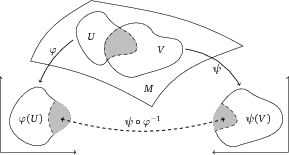
\includegraphics[width=\textwidth]{figures/fig_overlap_charts.png}
		\caption{Grafički prikaz manifolda M te transportnih funkcija $\varphi$ i $\psi$ od manifolda $M$ prema $\mathbb{R}^2$ te prikaz kompozicije transportnih mapa kao vezu između slika preklopnih dijelova $\Ua$ i $\Va$ u Euklidskom prostoru.}
	\end{figure}

\section{Tangencijalni prostor na manifoldu}

	Neka je M manifold. Tada se može konstruirati vektorski prostor nad $\mathbb{R}$ na slijedeći način: $(\boldsymbol{C}^\infty(M), +, \cdot)$, gdje je $\boldsymbol{C}^\infty(M) = \{ f: M \rightarrow \mathbb{R} \ | f \,je\, glatka\}$. Dakle, definiran je vektorski prostor kao skup svih glatkih mapa $f$ sa pridruženim operatorima zbrajanja i množenja. 
	
	\subsection{Krivulja na manifoldu} Neka je definirana krivulja na manifoldu kao glatka mapa $\gamma:\mathbb{R} \rightarrow M$, gdje je $\mathbb{R}$ promatran kao 1-dimenzionalni manifold.
	
	\subsection{Operator usmjerene derivacije} Neka je $\gamma: \mathbb{R} \rightarrow M$ glatka krivulja kroz točku $p\in M$ te bez gubljenja općenitosti može se uzima se da vrijedi $\gamma(0) = p$. Tada se može definirati operator usmjerene derivacije duž krivulje $\gamma$ u točki $p$ kao mapu na slijedeći način: \\
	\begin{gather}
		X_{\gamma, p} : \boldsymbol{C}^\infty(M) \rightarrow R \\
		f \mapsto (f \circ \gamma)'(0)
	\end{gather}
	Bitno je primijetiti kako je kompozicija $(f \circ \gamma)$ mapiranje unutar realnog prostora tako da se toj funkciji na uobičajan način može pronaći i evaluirati derivacija.
	Intuitivno gledano $X_{\gamma, p}$ je brzina krivulje $\gamma$ u točki $p$.
	
	\subsection{Tangencijalni prostor} Neka je M manifold koji sadrži točku $p$. Tada je tangencijalni prostor vektorski prostor nad $\mathbb{R}$ sa skupom operatora usmjerene derivacije tako da vrijedi: \\
	$T_p M := \{ X_{\gamma, p} \, | \, \gamma \, je \, glatka \, krivulja \, kroz \, p\}$ te sa nadodanim operatorima zbrajanja i skalarnog množenja.
	
	\begin{figure}[h!]
		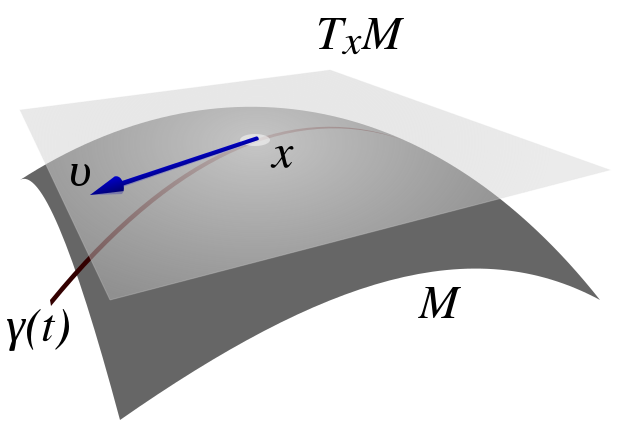
\includegraphics[width=\textwidth]{figures/txm.png}
		\caption{Na slici je prikazan manifold M. Parametrirana krivulja $\gamma(t)$ koja prolazi točkom $x$. Tangencijalni prostor manifolda M u točki x $T_x M$ te vektor usmjerene derivacije $v$ krivulje $\gamma (t)$ u točki $x$. }
	\end{figure}
	
\chapter{Lijeve grupe i Lijeva algebra}

	\paragraph{}Lijeva teorija je od velike važnosti i u fizici i u diferencijalnoj geometriji. U ovom dijelu bit će predstavljen koncept Lijeve grupe te pripadajuće Lijeve algebre. Fokus će biti usmjeren prema Specijalnim Euklidskim grupama SE(3) budući da su one predmet zanimljive u kontekstu ovog rada.
	
\section{Lijeve grupe}

	\paragraph{} Lijeva grupa je grupa $(G, \bullet)$ gdje je G glatki manifold klase $\boldsymbol{C}^\infty$, a $\bullet$ pripadajući operator nad G. Svojstva operatora $\bullet$ su slijedeća: 
	\begin{enumerate}
		\item Asocijativnost: $\forall a, b, c \in G :  a\bullet(b\bullet c) = (a\bullet b) \bullet c$
		\item Neutralni element: $\exists e \in G : \forall g \in G : g \bullet e = e \bullet g = g$
		\item Inverz: $\forall g \in G : \exists g^{-1} \in G : g \bullet g^{-1} = g^{-1} \bullet g = e$
	\end{enumerate}
	Ako vrijedi i svojstvo komutativnosti: $a \bullet b = b \bullet a, \forall a, b \in G$ tada je grupa abelijanska. Dana je toplogija nad G preko slijedećih mapa:
	
	\begin{gather}
		\mu: G \times G \rightarrow G \\
		(g_1, g_2) \mapsto g_1 \bullet g_2 \\ g_1, g_2 \in G
	\end{gather}
	
	i: 
	\begin{gather}
		i: G \rightarrow G \\
		g \mapsto g^{-1} \\
		g \in G
	\end{gather}
	
	Mape $g$ i $i$ su glatke mape. Dakle Lijeve grupe su topološke grupe, čiji se elementi unutar toploškim prostorom, odnosno dio manifolda, a operacija nad grupom $\bullet$ je kontinuirana, kao i njen inverz.

	\newpage
	\clearpage
	
\section{Specijalna euklidska grupa - SE(3)}

	\paragraph{}U ovom dijelu bit će definirano nekoliko različitih Lijevih grupa s konačnim ciljem definiranja specijalne ortogonalne grupe SO(3) te njenog proširenja na specijalnu Euklidsku grupu SE(3). 	
	
	\subsection{N-dimenzijska translacijska grupa} Mapa $\varphi$ je kruta mapa ako vrijedi 
	$\forall v, w \in \mathbb{R}^n, \, d(\varphi(v), \, \varphi(w)) = d(v, w)$. Drugim riječima mapa je kruta ako su nakon mapiranja duljine očuvane. \\
	Neka je skup $G$ sačinjena od svih krutih mapa tako da vrijedi $G = \{ \varphi: \mathbb{R}^n \rightarrow \mathbb{R}^n \, | \, \varphi\, je\, kruta\, mapa\} := T(n)$. Ako se skupu $T(n)$ pridruži operator kompozicije tada se dobiva translacijska Lijeva grupa $(T(n), \circ)$.
	
	\subsection{Opća linearna grupa (\textit{"General linear group"})} Neka je skup G sačinjen od matrica, tj. mapa $\varphi$ tako da vrijedi $G = \{ \varphi: \mathbb{R}^n \rightarrow \mathbb{R}^n \,|\, det \, \varphi \neq 0 \}:=GL(n, \mathbb{R}^n)$. Ako bi tome skupu pridodali operator kompozicije $\circ$ tada možemo definirati Lijevu grupu $(GL(n, \mathbb{R}^n), \circ)$. To je dakle grupa svih invertibilnih matrica koje svoje karakteristike glatkog manifolda naslijeđuju činjenicom da su takve matrice otvoreni podskup grupe svih nxn matrica $\mathbb{R}^{n^2}$ koje čine glatki manifold.
	
	\subsection{(Specijalna) Ortogonalna grupa} Neka je skup G sačinjen od matrica $Q$ tako da vrijedi \\ 
	$G = \{ Q \in GL(n, \mathbb{R}^n) \,|\, det \, Q = \pm 1\} := O(n)$. Budući da su matrice elementi skupa $GL(n, \mathbb{R}^n)$ njima se može pridodijeliti i naslijeđeni operator $\circ$. Takva Lijeva grupa $(O(n),\circ)$ zove se ortogonalna grupa. \\
	Specijalna ortogonalna grupa $SO(n)$ je podgrupa ortogonalnoj grupi, uz uvjet da matrice moraju imati determinante jednake 1. Ta grupe se ujedno naziva i rotacijska grupa jer sadrži sve rotacijske matrice. \\
	Obje grupe lančano naslijeđuju karakteristike glatkog manifolda od opće linearne grupe.
	
	\subsection{(Specijalna) Euklidska grupa} Euklidska grupa kao podgrupe sadrži translacijsku Lijevu grupu $T(n)$ i ortogonalnu grupu $O(n)$. Svaki element u $E(n)$ sastoji se od translacije koju slijedi ortogonalna transformacija. \\
	Specijalna Euklidska grupa kao podskup umjesto ortogonalne grupe sadrži specijalnu ortogonalnu grupu. U tom slučaju svaki član te grupe sadrži translaciju koju slijedi rotacija. Elementi te grupe su (n+1)x(n+1) matrice slijedećeg oblika: \\
	
	\begin{equation}
		\left \{
		\begin{bmatrix}
		R_{3 \times 3} & v_{3 \times 1} \\
		0 & 1
		\end{bmatrix}
		\, \Biggr\rvert \, R \in SO(3) \, , \, v \in \mathbb{R}^n
		\right \} \in SE(3)
	\end{equation}	

\section{Lijeva algebra}

	\subsection{Algebra} Algebra nad poljem K je skup od četiri elemenata $(A, +, \cdot, \bullet)$, gdje je $(A, +, \cdot)$ vektorski prostor nad poljem K, a $\bullet$ je produkt nad A, tj. bilinearno mapiranje: $\bullet : A \times A \rightarrow A$. \\
	Algebra $(A, +, \cdot, \bullet)$ može biti:
	\begin{enumerate}
		\item Asocijativna ako vrijedi $\forall v, w, z \in A : v \bullet (w \bullet z) = (v \bullet w) \bullet z$
		
		\item Unitalna ako vrijedi $\exists e \in A : \forall v \in A : e \bullet v = v \bullet e = v$
		
		\item Komutativna ili abelijanska ako vrijedi $\forall v, w \in A : v \bullet w = w \bullet v$
	\end{enumerate}
	
	\subsection{Lijeva algebra} Lijeva algebra je algebra čiji operator je Lijeva zagrada $[-,-]$ (tipično zvana komutator) za koju vrijede svojstva: 
	
	\begin{enumerate}
		
		\item Antisimetričnost: $\forall v \in A: [v, v] = 0$
		
		\item Jakobijev identitet: $\forall v, w, z \in A : [v,[w, z]] + [w,[z,v]] + [z,[v,w]] = 0$
		
	\end{enumerate} 
	
	Iz uvjeta o antisimetričnosti odmah vrijedi $[v,w]=-[w,v]$. Kod asocijativnih algebri komutator se definira kao $[v,w]:=v \bullet w - w \bullet v$.
	
	\subsection{Lijeva algebra Lijeve grupe} Svaka Lijeva grupa ima svoju pripadajuću Lijevu algebru. Lijeva algebra $g$ od Lijeve grupe $G$ je tangencijalni prostor oko točke identiteta $T_e G$.
	
	\subsection{Eksponencijalna mapa} Poveznica između Lijeve grupe i njene pripadajuće Lijeve algebre je eksponencijalna mapa. Ona je definirana na slijedeći način: $exp: T_eG \rightarrow	G$, tj. $exp: g \rightarrow G.$ \\ Postoji i logaritamska mapa koja služi za inverno mapiranje od Lijeve grupe prema pripadajućoj algebri.

\section{Algebra specijalne ortogonalne grupe $so(3)$}

	Naposlijetku bit će potrebno definirati pripadajuću Lijevu algebru $so(3)$ nad Lijevom grupom SO(3). \\
	Lijeva algebra $so(3)$ je skup anti-simetričnih realnih matrica. Budući da je takav skup matrica proizašao iz tangencijalnog prostora rotacijske grupe SO(3) tada će te matrice zapravo predstavljati tenzore kutnih brzina oko neke konfiguracije $R$. \\
	Na primjer, ako je rotacija ua kut $\psi$ oko z-osi definirana kao:
	
	\begin{equation}
		R( \hat{e}_3, \psi ) = 
		\begin{bmatrix}
			cos(\psi)	&	-sin(\psi)	&	0 \\
			sin(\psi)	&	cos(\psi)	&	0 \\
			0			&	0			&	1 \\	
		\end{bmatrix} \in SO(3)
	\end{equation}
	
	Ako se sada razvije matrica rotacije u Taylorov red prvog stupnja dobit će se matrica infinitiezimalne rotacije: \\
	\begin{equation}
		R( \hat{e}_3, \partial \psi ) = I + \partial \psi 
		\begin{bmatrix}
			0	&	-1	&	0 \\
			1	&	0	&	0 \\
			0	&	0 	&	0
		\end{bmatrix}
		= I + \partial \psi J_z
	\end{equation}
	\\
	\noindent Gdje je $J_z$ jedan od tri elementa koja definiraju bazu algebre $so(3)$. Ostali elementi baze su:
	
	\begin{equation}
		J_1 = 
		\begin{bmatrix}
		0	&	0	&	0 \\
		0	&	0	&	-1 \\
		0	&	1 	&	0
		\end{bmatrix} \\
		\, , \, J_2 = 
		\begin{bmatrix}
		0	&	0	&	1 \\
		0	&	0	&	0 \\
		-1	&	0 	&	0
		\end{bmatrix} 
	\end{equation}
	\\
	Još se nazivaju i generatori rotacije jer njihovim uzastopnim primjenjivanjem se postiže rotacija za željeni kut na slijedeći način:
	
	\begin{align}
		R( \hat{e}_3, \psi ) & = (I + \partial \psi J_z)^n \\
							 & = \lim_{n \rightarrow \infty} \left (I + J_z \frac{\psi}{n} \right )^n \\
							 & = e^{J_z \psi}
	\end{align}
	\\
	Iz gornje relacije se također vidi veza između matrice rotacije, elementa grupe SO(3), i generatora infinitezimalne rotacije, elementa algebre ($so(3)$), preko prethodno definirane eksponencijalne mape. \\
	Sada se može definirati opća rotacija oko vektora $\hat{n}$ za kut $\psi$ kao:
	
	\begin{equation}
		R( \hat{n}, \phi ) = e^{(J_1 n_1 + J_2 n_2 + J_3 n_3)\psi}
	\end{equation}
	\\
	Uzevši to u obzir, vektor kutne brzine $\vec{\omega} = [\omega_x, \omega_y, \omega_z]$, može se zapisati u obliku tenzora, tj. elementa algebre $so(3)$ kao: 
	
	\begin{equation}
		\hat{\omega} = 
		\begin{bmatrix}
			0			&	-\omega_z	& 	\omega_y \\
			\omega_z	&	0			& 	-\omega_x \\
			-\omega_y	&	\omega_x	&	0
		\end{bmatrix} \, , \, \hat{\cdot}: \mathbb{R}^3 \rightarrow so(3)
	\end{equation}
	
	\noindent Gdje kapa-operator mapiranje iz Realnog 3-dimenzionalnog prostora prema Lijevoj algebri $so(3)$. Njemu inverzan operator je v-operator koja je definirana kao $\check{\cdot}:so(3) \rightarrow \mathbb{R}^3$.
	
\chapter{Matematički model letjelice}

\paragraph{}U ovom radu kao sustav upravljanja razmatra se multirotorska letjelica sa četiri rotora postavljena u plus konfiguraciju. Kao pomoć pri prikazivanju jednadžbi odabrana su dva koordinatna sustava: 
\begin{itemize}
	\item Globalni: $\{\vec{e}_1, \vec{e}_2, \vec{e}_3\}$
	\item Lokalni - tijelo letjelice: $\{\vec{b}_1, \vec{b}_2, \vec{b}_3\}$
\end{itemize}

\noindent Općenite jednadžbe gibanja takvog sustava su:
\begin{gather}
	\dot{x} = v \\
	m \dot{v} = mge_3 - fRe_3 \label{thrust_dyn}\\
	\dot{R} = R\hat{\Omega} \label{model_ang} \\
	J\dot{\Omega} + \Omega \times J\Omega = M 
\end{gather}

gdje je:
\begin{itemize}
	\item $x \in \mathbb{R}^3$ - trenutna pozicija letjelice
	
	\item $m \in \mathbb{R}$ - ukupna masa letjelice
	
	\item $f \in \mathbb{R}$ - ukupni potisak letjelice 
	
	\item $R \in SO(3)$ - matrica rotacije iz lokalnog u globalni koordinatni sustav
	
	\item $\Omega \in \mathbb{R}^3$ - kutna brzina letjelice u lokalnom koordinatnom sustavu
	
	\item $J \in \mathbb{R}^{3\times3}$ - matrica inercije letjelice s obzirom na lokalni koordinatni sustav
	
	\item $M \in \mathbb{R}^3$ - ukupni moment letjelice s obzirom na lokalni koordinatni sustav
\end{itemize}

\noindent Budući da se upravlja brzinom vrtnje rotora potrebna je poveznica sa ukupnom silom i ukupnim momentima. Ta dva pojma povezana su preko sile koju generira pojedini rotor $f_i$, a veza je slijedeća:

\begin{gather}
	f_i = \zeta_i b_f \Omega_{i}^2 \\
	M_i = b_m f_i
\end{gather}

gdje je:
\begin{itemize}
	\item $\zeta_i = 1,\, i = 2, 4$, $\zeta_i = -1,\, i=1,3$ zbog različitih smjerova vrtnje rotora
	\item $b_f$ - konstanta potiska motora
	\item $b_m$ - kontatnta momenta motora
\end{itemize}

\newpage
\clearpage

Radi lakše pretvorbe uvodi se matrični zapis na slijedeći način: 

\begin{equation}
	\begin{bmatrix}
		f \\
		M_1 \\
		M_2 \\
		M_3 
	\end{bmatrix} 
	=
	\begin{bmatrix}
		1	&	1	&	1	&	1 \\
		0	&	d	&	0	&	-d \\
		-d 	&	0	&	d	&	0 \\
		b_m &	-b_m	& 	b_m	& -b_m
	\end{bmatrix}
	\cdot
	\begin{bmatrix}
		f_1 \\
		f_2 \\
		f_3 \\
		f_4
	\end{bmatrix}
\end{equation}

\begin{figure}[h!]
	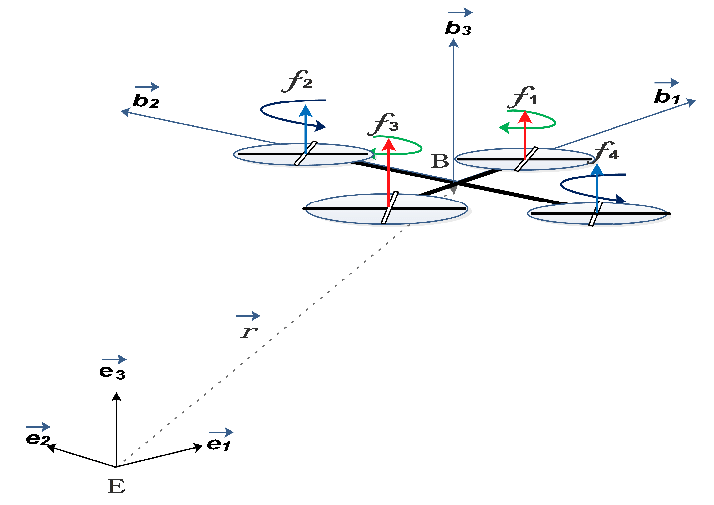
\includegraphics[width=\textwidth]{figures/model.png}
	\caption{Vizualni prikaz letjelice i koordinatnih osi.}
\end{figure}

\noindent U ovom radu bit će razmotren konkretan model multirotorske letjelice sa benzinskim motorima u Gazebo simulatoru. U nastavku će biti izloženi fizikalni parametri letjelice koji su potrebni za geometrijsko upravljanje.

\begin{longtable}[c]{| c | c |}
	\caption{Tablica parametera rotora.\label{long}} \\
	\hline
	\multicolumn{2}{| c |}{Parametri rotora} \\	
	\hline
	Masa rotora & 0.2 kg \\
	\hline
	Radius rotora & 0.33 m \\
	\hline
	Konstanta potiska motora & 0.000456874 kg$\cdot$m \\
	\hline
	Konstanta momenta motora & 0.01 m \\
	\hline
	Vremenska konstanta motora & 0.125 \\
	\hline
\end{longtable}

\newpage
\clearpage

\begin{figure}[h!] 
	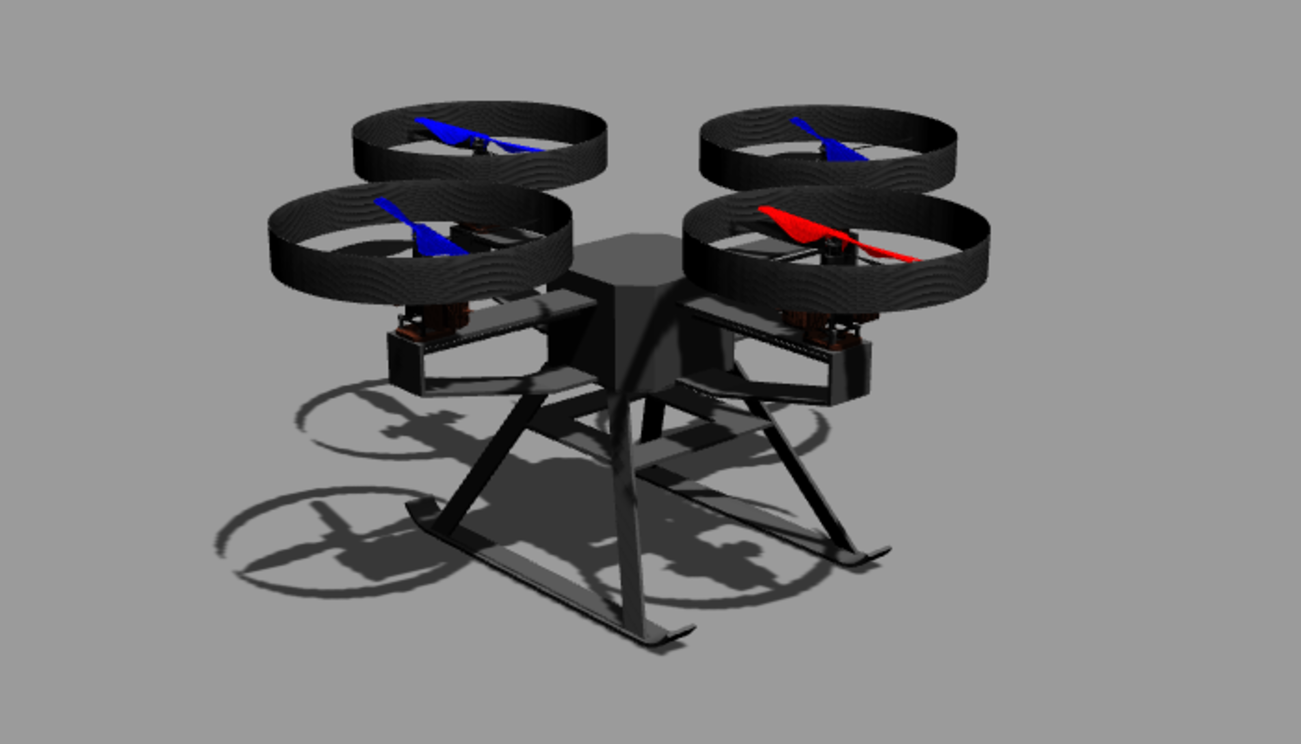
\includegraphics[width=15cm, height=10cm]{figures/morus_crop.png}
	\centering
	\caption{Model letjelice u Gazebo simulatoru.}
\end{figure}

\begin{longtable}[c]{| c | c |}
	\caption{Tablica parametera tijela letjelice.\label{long}} \\
	\hline
	\multicolumn{2}{| c |}{Parametri tijela letjelice} \\	
	\hline
	Masa letjelice & 30 kg \\
	\hline
	Moment inercije letjelice u x smjeru  & 5.5268 $\text{kg} \cdot \text{m}^2$ \\
	\hline
	Moment inercije letjelice u y smjeru & 5.5268 $\text{kg} \cdot \text{m}^2$ \\
	\hline
	Moment inercije letjelice u z smjeru & 6.8854 $\text{kg} \cdot \text{m}^2$ \\
	\hline
	Duljina kraka & 0.515 m \\
	\hline
\end{longtable}

\chapter{Geometrijsko upravljanje}
	
	\paragraph{}Ako se pri upravljanju sustavima njegov konfiguracijski prostor, odnosno njegove varijable stanja, shvaća kao glatki manifold tada se govori o geometrijskom upravljanju sustavima. Kao što je već rečeno, jedna od prednosti pri upravljanju u prostoru manifolda jest koordinatna invarijantnost. Nakon što je odabran i fiksiran početni koordinatni sustav svo daljnje upravljanje je neovisno o trenutnoj konfiguraciji sustava. \\
	Neka je definiran sustav:
	
	\begin{equation}
		\dot{x}=f(x), \, x \in M
	\end{equation}
	Uvodi se pojam vektorskih polja kao skup svih mapa od manifolda M prema TM, odnosno tangencijalnom svežnju (unija svih tangencijalnih prostora $T_xM ,\, \forall x\in M$). \\
	Tada je f jedno vektorsko polje, tj. glatka mapa od manifolda prema tangencijalnom prostoru $T_xM$. Dakle dinamički sustav je vektorsko polje, tj. određen je tokom samo jednog vektorskog polja i ovisi o početnim uvjetima. Pod tokom vektorskog polja misli se na krivulju $x(t)$ kao rješenje sustava. \\
	Kako bi se upravljalo dinamičkim sustavom mora se uzeti u obzir familija vektorskih polja $f(\cdot, u)$ parametrirana sa upravljačkom varijablom $u$. \\
	\begin{equation}
		\dot{x} = f(x(t),\, u(t)), \, x(t)\in M, \, u(t)\in \Ua \subset \mathbb{R}^m
	\end{equation}
	\begin{figure}[h!]
		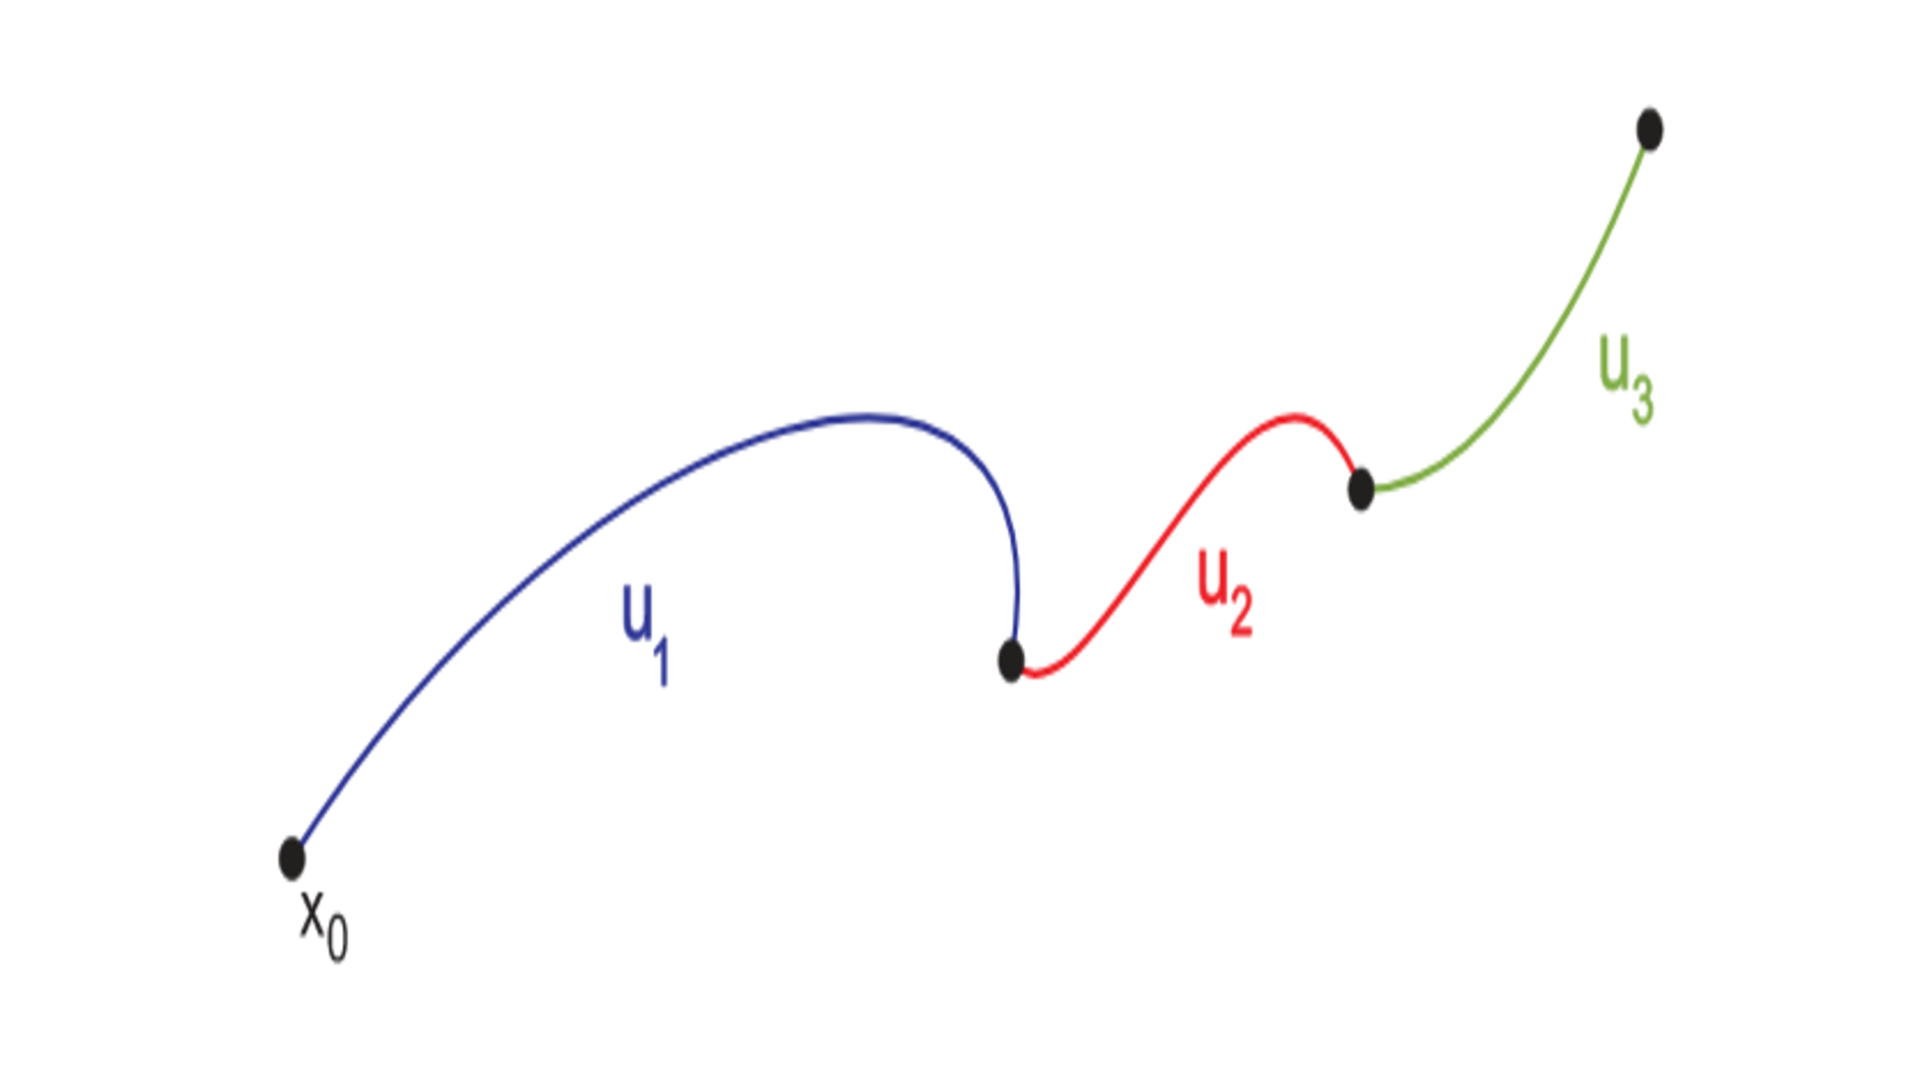
\includegraphics[width=\textwidth, height=5cm]{figures/krivulja.png}
		\caption{Krivulja rješenja sustava uz dodane upravljačke funkcije $u_1(t)$, $u_2(t)$ i $u_3(t)$}
	\end{figure}
	
	\newpage
	\clearpage
	
\section{Geometrijsko upravljanje letjelicom}
	
	\paragraph{}Ukoliko se promatra sustav letjelice tada su varijable stanja razvijene na manifoldu Lijeve grupe SE(3), njihove derivacije leže na vektorskim poljima, odnosno tangencijalnom svežnju koji tada čini Lijevu algebru $se(3)$. Dakle elementi Lijeve grupe predstavljat će konfiguracije, tj. orijentaciju i pomak sustava letjelice dok elementi Lijeve algebre će predstavljati njene kutne, odnosno linearne brzine. \\
	Jedna od prednosti ovakvog načina upravljanja javlja se prilikom prikaza orijentacije sustava pomoću rotacijske matrice koja jasno definira vektore lokalnog koordinatnog sustava. Kod klasičnog upravljanja korištenjem Eulerovih kuteva javljaju se singulariteti. Ako je definiran neki redoslijed rotacija oko osi (npr. $x \rightarrow y \rightarrow z$) te ako je druga po redu rotacija za kut 90 ili 270 tada se dešava tzv. \textit{"Gimbal lock"}. U tom trenutku se gubi 5jedan stupanj slobode, odnosno preostale dvije rotacije se odvijaju oko iste osi.
	
	\begin{figure}[h!]
		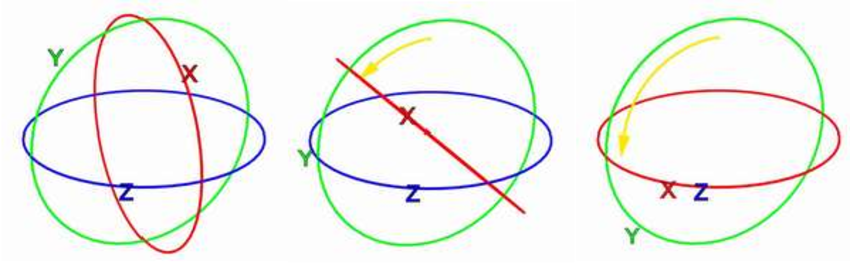
\includegraphics[width=\textwidth]{figures/gimbal_lock.png}
		\caption{Prikaz preklapanja osi prilikom Eulerovih rotacija. Na desnoj slici može se vidjeti kako će rotacije oko x i z osi biti istovjetne.}
	\end{figure}
	
	\noindent Prilikom predstavljanja orijentacije putem kvaterniona ne javlja se problem singulariteta, ali zato se pojavljuje problem dvosmislenosti. Drugim riječima kvaternioni $q$ i $-q$ predstavljaju isti kvaternion, odnosno istu rotaciju u prostoru. Opisani problemi ne pojavljuju se prilikom predstavljanja orijentacije sustava kao element Lijeve grupe SO(3). \\
	Geometrijsko upravljanje letjelicom svodi se na izračunavanje ukupne sile potiska svih rotora te momenata oko osi lokalnog sustava na temelju zadanih vrijednosti pozicije, linearne brzine i akceleracije, odnosno orijentacije, kutne brzine i akceleracije. Sama struktura regulatora je kaskadna, prvo se računa smjer i ukupni iznos sile potiska na temelju pozicijskih referenci te zatim momenti na temelju orijentacijskih referenci. Naposlijetku se dobivene upravljačke vrijednosti sile potiska i momenata preračunavaju u brzine zakreta rotora kako bi se mogle primijeniti na sustav letjelice.

	\newpage
	\clearpage

	\begin{figure}[h!]
		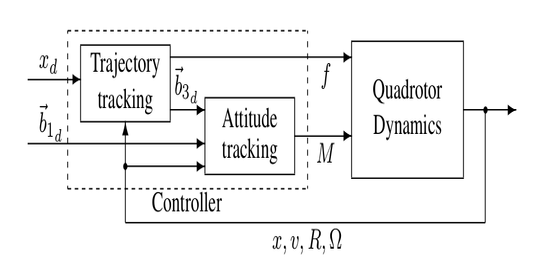
\includegraphics[width=\textwidth, height=5cm]{figures/controller.png}
		\caption{Prikaz kaskadne strukture geometrijskog kontrolera.}
	\end{figure}
	
	U nastavku bit će prikazana sinteza upravljčkog zakona, no najprije će biti potrebno definirati funkcije pogreške. To će biti lako napraviti za praćenje pozicije budući da je se ono odvija unutar translacijske grupe T(3) čiji su elementi dio $\mathbb{R}^3$. Pogreške orijentacije i kutne brzine bit će potrebno pažljivo definirati budući da leže unutar grupe SO(3), odnosno unutar njenog tangencijalnog prostora.
	
\section{Pogreške praćenja reference}

	\paragraph{}Prije nego se započne sinteza geometrijskog regulatora potrebno je definirati funkcije pogrešaka pozicije, orijentacije te linearne i kutne brzine s obzirom na željenu vrijednost (u ostatku teksta takvi simboli sadrži d - \textit{desired} u subskriptu) i trenutnu vrijednost.
	
	\noindent Kako bi se definirale pogreške orijentacije i kutne brzine nad prostorom grupe SO(3) bit će potrebno uvesti nekoliko pojmova.
	\subsection{Funkcija pogreške praćenja reference} Neka je Q manifold. Tada se definira funkcija pogreške konfiguracije $\Psi : Q \times Q \rightarrow \mathbb{R}$. Neka je takva funkcija simetrična: $\Psi(q, r) = \Psi(r, q), \, \forall q,r\in Q$ te se definira korištenje funkcije sa fiksnom (referentnom) konfiguracijom $r$ kao $\Psi_r(q) = \Psi(q, r)$. \\
	Nadalje definirani su diferencijali s obzirom na prvi i drugi argument kao: 
	\begin{gather}
		d_1 \Psi (q, r) = d \Psi_r(q) \in T_q Q \\
		d_2 \Psi (q, r) = d \Psi_q(r) \in T_r Q
	\end{gather}
	
	\newpage
	\clearpage
	Sada se može definirati pogreška praćena reference oko neke konfiguracije $r\in Q$ kao glatka, simetrična i omeđena funkcija pogreške konfiguracije za koju vrijedi: 
	\begin{enumerate}
		\item $\Psi(r,r)=0$
		
		\item $d_1 \Psi(r, r) = 0$
		
		\item $\text{Hess}_1\Psi (r, r)\text{ je pozitivno definitan}$
	\end{enumerate}
	
	\subsection{Prijenosna mapa} Neka se na manifoldu $Q$ se nalaze dvije krivulje brzine za koje vrijedi $\gamma'(t_0)=q$ i $\gamma_{ref}'(t_0)=r$. Kako bi uveli pojam pogreške brzine potrebno je moći usporediti takve dvije krivulje. Budući da one leže u različitim tangencijalnim prostorima $T_r Q$ i $T_q Q$ potrebno je uvesti mapu pomoću koje će se moći provesti ta usporedba. Definira se prijenosna mapa $\Ta(q,r): T_r Q \mapsto T_q Q$.
	
	\subsection{Funkcija brzine pogreške praćenja reference} Neka je uzet par koji sačinjava funkcija pogreške praćenja reference i pripadna prijenosna mapa $(\Psi, \Ta)$. Takav par se definira kao kompatibilan ako vrijedi:
	\begin{equation}
		d_2\Psi(q,r) = - \Ta(q,r)(d_q\Psi(q,r))
	\end{equation}
	\noindent Nadalje Lijeva derivacije funkcije pogreške slijeđenja reference definira se na slijedeći način:
	\begin{equation}
		\La_{X_q, Y_r}\Psi(q,r) = d_1\Psi(q,r) \cdot X_q + d_2\Psi(q,r) \cdot Y_r
	\end{equation}
	\noindent Ako se primijeni Lijeva derivacija i uvjet kompatibilnosti na funkciju pogreške praćenja reference tada se dobije slijedeća relacija:
	\begin{align}
		\frac{d}{dt} \Psi(\gamma(t), \eta(t)) &= d_1\Psi(\gamma(t), \eta(t)) \cdot \gamma '(t) + d_2\Psi(\gamma(t), \eta(t)) \cdot \eta ' (t)\\
		&= d_1\Psi(\gamma(t), \eta(t)) \cdot \gamma '(t) + (- \Ta(\gamma(t), \eta(t))(d_1\Psi(\gamma(t), \eta(t)) \cdot \eta'(t)) \\
		&= d_1\Psi(\gamma(t), \eta(t)) \cdot (\gamma '(t) - \Ta(\gamma(t), \eta(t))\eta'(t)) \label{error}\\
		&= d_1\Psi(\gamma(t), \eta(t)) \dot{e}(t)
	\end{align}
	Dakle, kao pogreška brzine između krivulja $\gamma$ i $\eta$ odabire se $\dot{e}(t)$, a za pogrešku u konfiguraciji uzimat će se diferencijal s obzirom na prvi argument funkcije pogreške praćenja reference $d_1\Psi(\gamma(t), \eta(t)$.
	
	\newpage
	\clearpage
	
	\subsection{Funkcije pogreške u SO(3) prostoru}
	Neka vrijedi da je $R := R(t)$ i $R_d := R_d(t)$. Na prethodno definiran način konstruiran je kompatibilan par $(\Psi_{SO(3)}(R, R_d), \Ta(R, R_d))$ koji glasi:
	\begin{gather}
		\Psi_{SO(3)}(R, R_d) = \frac{1}{2} tr[I - R_d^T R] \\
		\Ta(R, R_d) = R^T R_d
	\end{gather}
	
	Deriviranjem funkcije pogreške praćenja reference dobije se slijedeća relacija:
	\begin{equation}
		\frac{d}{dt} \Psi(R, R_d) = \frac{1}{2}(R_d^TR - R^TR_d)^{\text{V}} \cdot (\Omega - R^TR_d\Omega_d)
	\end{equation}
	
	Gdje su kao pogreška konfiguracije $e_R$ i pogreška slijeđenja kutne brzine odabrane kao: 
	\begin{gather}
		e_R(R, R_d) = \frac{1}{2}(R_d^TR - R^TR_d)^{\text{V}} \label{e_R}\\
		e_{\Omega}(R, \Omega, R_d, \Omega_d) = \Omega - R^TR_d\Omega_d \label{e_omega}
	\end{gather}
	Izvod se nalazi u dodatku.
	
	\subsection{Funkcije pogreške u T(3) prostoru}
	Budući da je translacijska grupa definirana nad $\mathbb{R}^3$ prostorom, funkcije pogreške linearne pozicije i brzine su jasno definirane i glase:
	\begin{gather}
		e_x = x - x_d \\
		e_v = v - v_d \label{e_v}
	\end{gather}
	
	\newpage
	\clearpage
	
\section{Upravljački zakon}

	Geometrijsko upravljanje bit će realizirano na dva načina: pozicijsko upravljanje i upravljanje orijentacijom. Kod pozicijskog upravljanja referentne vrijednosti podrazumijevat će poziciju - $x_d$ i vektor smjera x-osi koordinatnog sustava letjelice - $b_{1d}$. Referentna vrijednost pozicije bit će zadana u obliku kontinuiranog signala što znači da se mogu dobiti referentne vrijednosti brzine $v_d$ i akceleracije $a_d$. \\
	Referentne vrijednosti upravljanja orijentacijom su visina, te kompletna matrica rotacije koordinatnog sustava letjelice - $R_d$. Zadana matrica orijentacije također se promatra kao kontinuirani signal što znači da se posljedično mogu dobiti referentne vrijednosti kutne brzine $\Omega_d$ i kutne akceleracije $\alpha_d$. \\
	Budući da su oba upravljačka načina relativno slična, najprije će biti predstavljen pozicijski način upravljanja budući da on obuhvaća i upravljanje orijentacijom.  \\
	\subsection{Pozicijski način upravljanja}
	Upravljačke vrijednosti za ukupni potisak i momente u pozicijskom načinu upravljanja su slijedeće:
	\begin{gather}
		f = - (- k_x e_x - k_v e_v - mg e_3 + m \ddot{x}_d) \cdot Re_3 \label{thrust_ctrl} \\
		M = -k_R e_R - k_\Omega e_\Omega + \Omega \times J \Omega - J(\hat{\Omega}R^TR_c\Omega_c - R^TR_c\dot{\Omega}_c) \label{pos_moment}
	\end{gather}
	
	gdje su:
	\begin{itemize}
		\item $R_c \in SO(3)$ je izračunata orijentacija i iznosi $[\vec{b}_{1c}, \vec{b}_{3c} \times \vec{b}_{1c}, \vec{b}_{3c}]$ 
		\item $\Omega_c \in \mathbb{R}^3$ je izračunata kutna brzina letjelice 
		\item $\dot{\Omega}_c \in \mathbb{R}^3$ je izračunata kutna akceleracija letjelice
	\end{itemize}
	Budući da željeni smjer x-osi letjelice $b_{1d}$ ne mora uvijek ležati u na ravnini čija je normala vektor potiska letjelice potrebno je napraviti projekciju i normalizaciju željenog vektora smjera na spomenutu ravninu na slijedeći način:
	\begin{equation}
		b_{1c} = - \frac{1}{\Vert \vec{b}_{3c} \times \vec{b}_{1d} \Vert}(\vec{b}_{3c} \times (\vec{b}_{3c} \times \vec{b}_{1d}))
	\end{equation}
	Vektor potiska računa se na slijedeći način:
	\begin{equation}
		\vec{b}_{3c} = \frac{- k_x e_x - k_v e_v - mg e_3 + m \ddot{x}}{\Vert - k_x e_x - k_v e_v - mg e_3 + m \ddot{x} \Vert}
	\end{equation}
	
	\noindent Izračunata kutna brzina dobija se po uzoru na \ref{model_ang}:
	\begin{equation}
		\hat{\Omega}_c = R_c^T \dot{R}_c
	\end{equation} 
	
	\noindent Izračunata kutna akceleracija dobija se deriviranjem gornjeg izraza:
	\begin{align*}
		\dot{\hat{\Omega}} &= (\dot{R}_c^T \dot{R}_c) + (R_d^T \ddot{R}_c) \\
		&= (R_c \hat{\Omega}_c)^T(R_c\hat{\Omega}_c) + (R_c^T \ddot{R}_c) \\
		&= - \hat{\Omega}_c \hat{\Omega}_c + R_c^T \ddot{R}_c \numberthis
	\end{align*}
	Izvod upravljačkog zakona se nalazi u dodatku.
	
	\newpage
	\clearpage
	\subsection{Orijentacijski način upravljanja}
	Upravljanje orijentacijom podrazumijeva matricu rotacije koordinatnog sustava letjelice $R_d$ te željena vrijednost visine letjelice $x_{3d}$. 
	Upravljački zakon je vrlo sličan prethodnome i glasi:
	\begin{gather}
		f = \frac{k_x(x_3 - x_{3d}) + k_v(\dot{x}_3 - \dot{x}_{3d}) + mg - m\ddot{x}_{3d}}{e_3 \cdot Re_3} \label{orient_thrust} \\
		M = -k_R e_R - k_\Omega e_\Omega + \Omega \times J \Omega - J(\hat{\Omega}R^TR_d\Omega_d - R^TR_d\dot{\Omega}_d \label{orient_moment}
	\end{gather}
	gdje su:
	\begin{itemize}
		\item $\Omega_d \in \mathbb{R}^3$ je željena, tj. zadana kutna brzina letjelice 
		\item $\dot{\Omega}_d \in \mathbb{R}^3$ je željena, tj. zadana kutna akceleracija letjelice
	\end{itemize}
	
	\noindent Upravljački zakon za momente \ref{orient_moment} jednak je kao i onome u pozicijskom načinu upravljanja \ref{pos_moment}. Upravljački zakon za potisak \ref{orient_thrust} vrlo je sličan kao i u pozicijskom načinu upravljanja, sa razlikom da se ovdje jedino uzima u obzir visina te njene derivacije. Dobije se izravno iz \ref{thrust_dyn} ukoliko se razmatra samo treća komponenta vektora:
	\begin{equation}
		m\ddot{x}_3 = mg - f e_3 \cdot R e_3
	\end{equation}
	Uvrštavanje upravljačkog zakona \ref{orient_thrust} dobiva se linearni sustav drugog reda:
	\begin{equation}
		m\ddot{x}_3 = -k_x(x_3 - x_{3,d}) - k_v(\dot{x}_3 - \dot{x}_{3,d}) + m\ddot{x}_{3,d}
	\end{equation}
	Takav sustav bit će stabilan za pozitivne konstantne $k_x$ i $k_v$.
	
\chapter{Rezultati simulacije}

	\paragraph{}Simulacija ovakvog upraljanje bit će napravljena u Gazebo simulatoru unutar ROS okruženja. Upravljačka petlja implementirana je u C++ programskom jeziku za već opisanu multirotorsku letjelicu sa benzinskim motorima. \\
	U ovom dijelu naglasak je na slijeđenju trajektorije u pozicijskom načinu upravljanja, budući da je ovakav geometrijski kontroler primarno napravljen za slijeđenje trajektorije. Odzivi na skokovitu pobudu bit će također prikazani u oba načina upravljanja za male pobude. \\
	Odabrana frekvencija upravljačke petlje je 100 Hz. Prilikom računanja kutne brzine i kutne akceleracije uzeto je vrijeme diskretizacije od 10 ms. Postavljeni parametri regulatora nalaze se u dodatku. \\
	Zasićenja su postavljena na upravljačke vrijednosti momenata kako bi se izbjegli neželjeni skokovi. Također je postavljeno zasićenje nad izračunatim vrijednostima kutnih brzina i akceleracija, iz istog razloga.
	
	\section{Skokovita pobuda u pozicijskom načinu upravljanja}
	U ovom dijelu zadane su skokovite pobude na poziciju $x_d$. Željene linearne brzine i akceleracije nisu zadane. Skokovita pobuda će slijedno biti primijenjena redom po z, x te y smjeru.
	
	\begin{figure}[h!]
		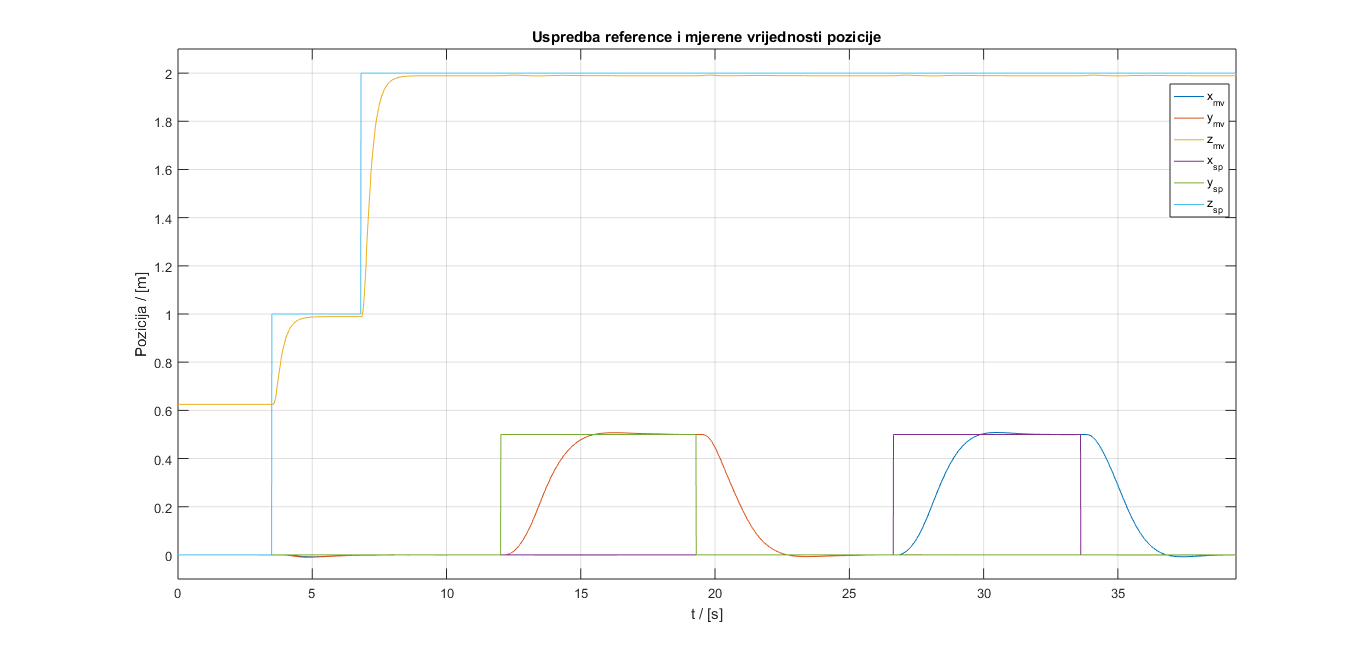
\includegraphics[width=\textwidth]{plots/pos_pos2.png}
		\caption{Prikaz odziva pozicija na skokovitu pobudu.}
	\end{figure}
	
	\newpage
	\clearpage
	
	\begin{figure}[!h]
		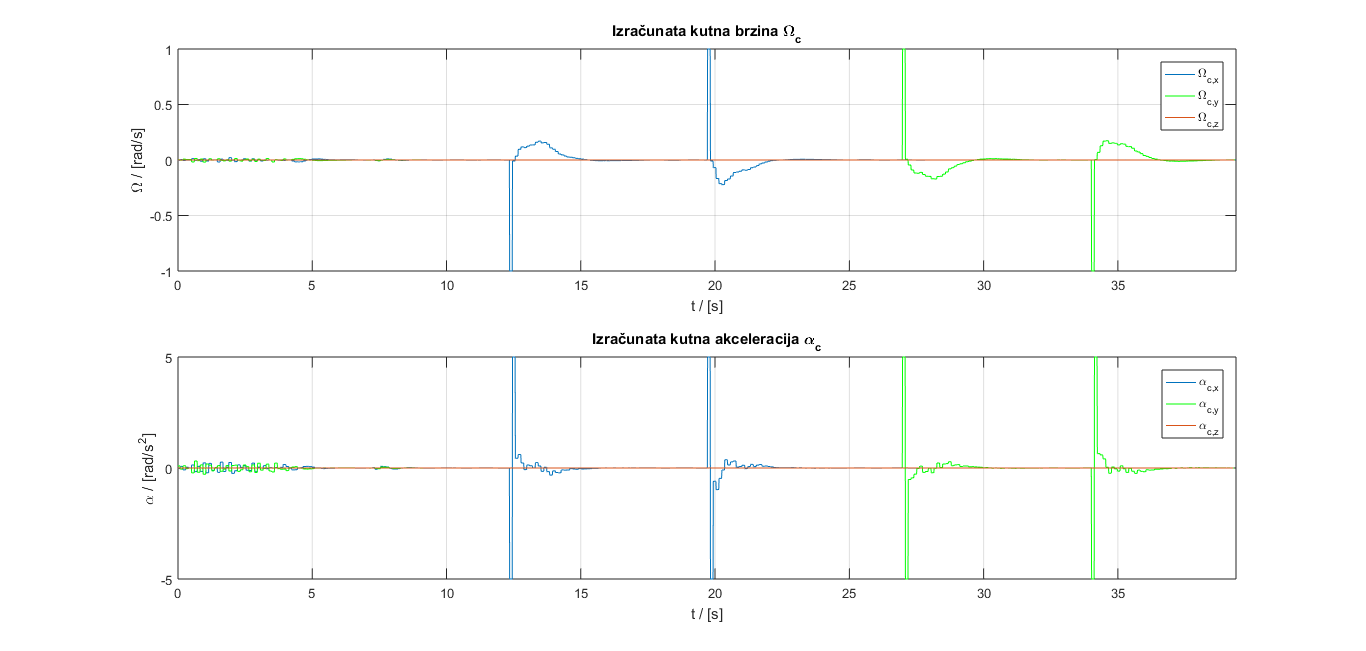
\includegraphics[width=\textwidth]{plots/pos_alpha_omega2.png}
		\caption{Prikaz izračunatih vrijednosti kutne brzine i kutne  akceleracije  tokom zadavanja skokovite pozicijske pobude.}
	\end{figure}
	
	\begin{figure}[h!]
		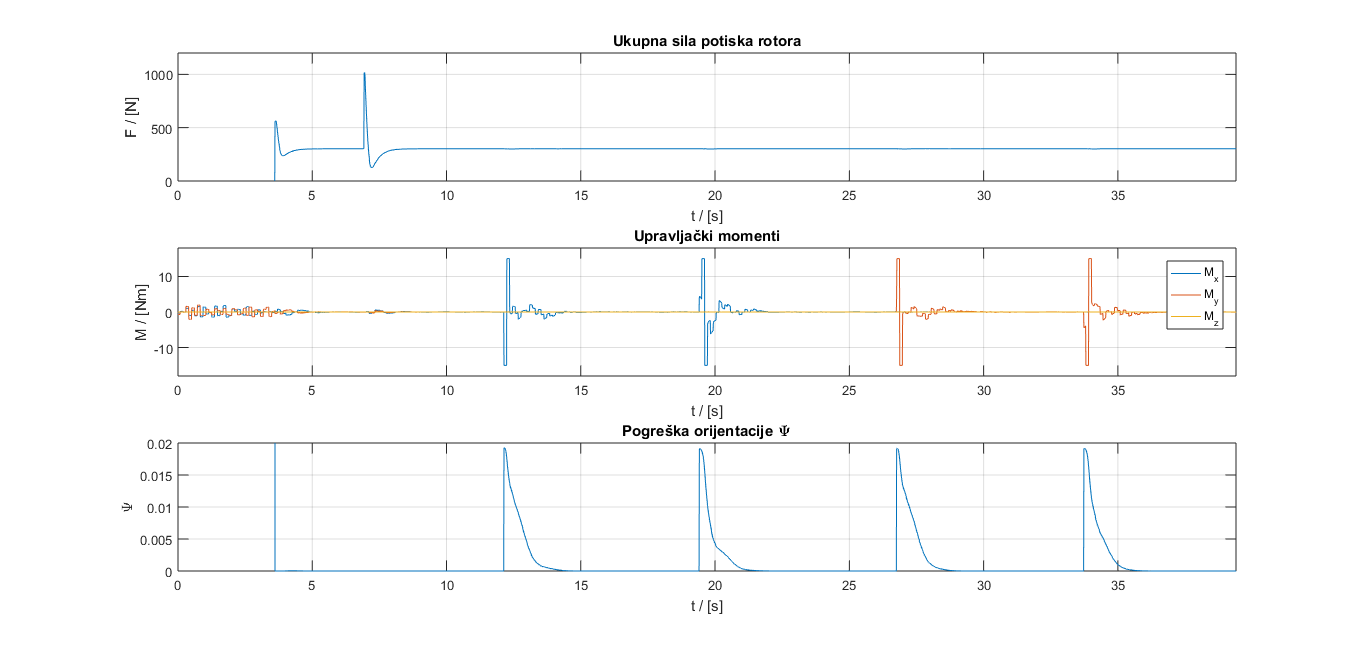
\includegraphics[width=\textwidth]{plots/pos_force_moments2.png}
		\caption{Prikaz upravljačkih vrijednosti sila i momenata te pogreške orijentacije tokom zadavanja skokovite pozicijske pobude.}
	\end{figure}
	
	Upravljanje orijentacijom također je dio pozicijskog upravljanja, pripadajući odzivi bit će prikazani u nastavku.
	
	\newpage
	\clearpage
	
	\begin{figure}[h!]
		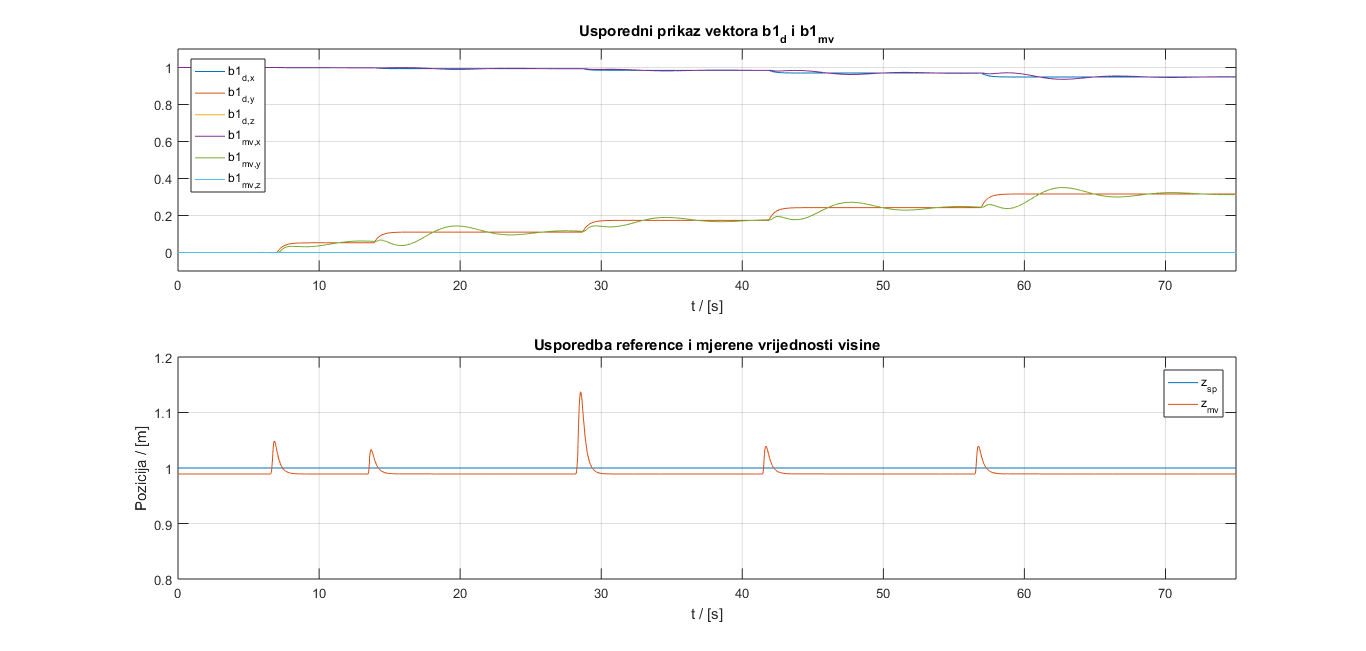
\includegraphics[width=\textwidth]{plots/b1d_b1d2.png}
		\caption{Prikaz odziva smjera x-osi letjelice na skokovitu pobudu.}
	\end{figure}

	\begin{figure}[!h]
		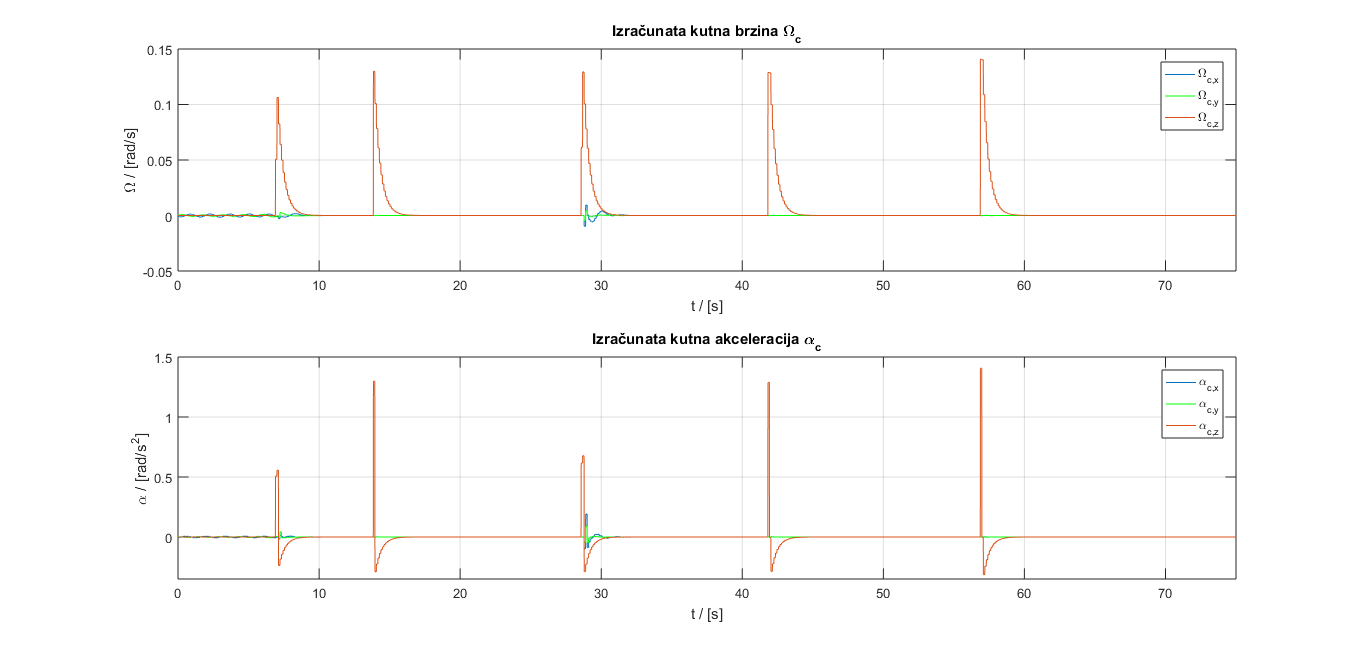
\includegraphics[width=\textwidth]{plots/b1d_alpha_omega2.png}
		\caption{Prikaz izračunatih vrijednosti kutne brzine i kutne  akceleracije tokom zadavanja skokovite pobude smjera x-osi letjelice.}
	\end{figure}
	
	Zadane pobude na orijentaciju x-osi su vrlo male. Prilikom velikih promjena željene vrijednosti $b1_d$, letjelica poprima velike vrijednosti momenta oko z-osi te sustav postaje nestabilan, što je za očekivati. 
	
	\newpage
	\clearpage
	
	\begin{figure}[h!]
		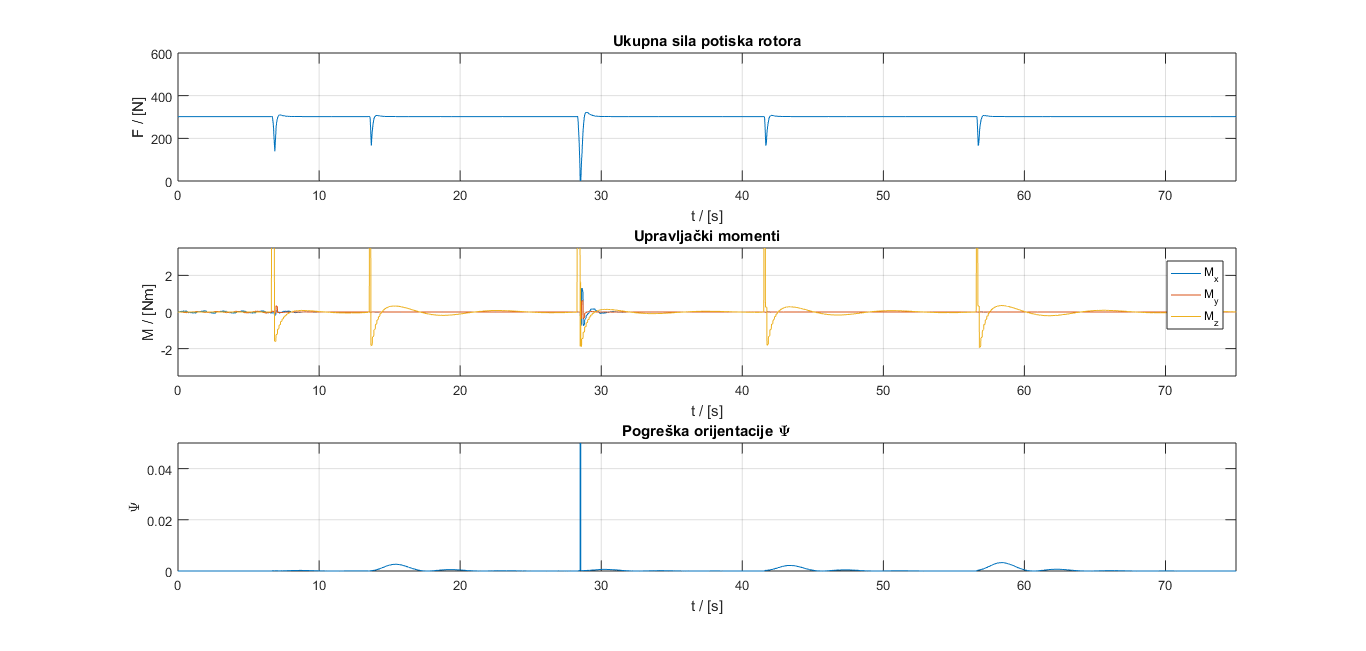
\includegraphics[width=\textwidth]{plots/b1d_force_moments2.png}
		\caption{Prikaz upravljačkih vrijednosti sila i momenata te pogreške orijentacije tokom zadavanja skokovite pobude smjera x-osi letjelice.}
	\end{figure}
	
	\section{Skokovita pobuda u orijentacijskom načinu upravljanja}
	U ovom dijelu bit će zadana željena orijentacijska matrica $R_d$ te željena visina $x_{d,3}$. Orijentacijska matrica će biti zadana na način da se slijedno uvrštavaju željeni kutevi poniranja, kotrljanja i skretanja od 10 stupnjeva. Željene kutne brzine i akceleracije neće biti zadane. 
	\begin{figure}[h!]
		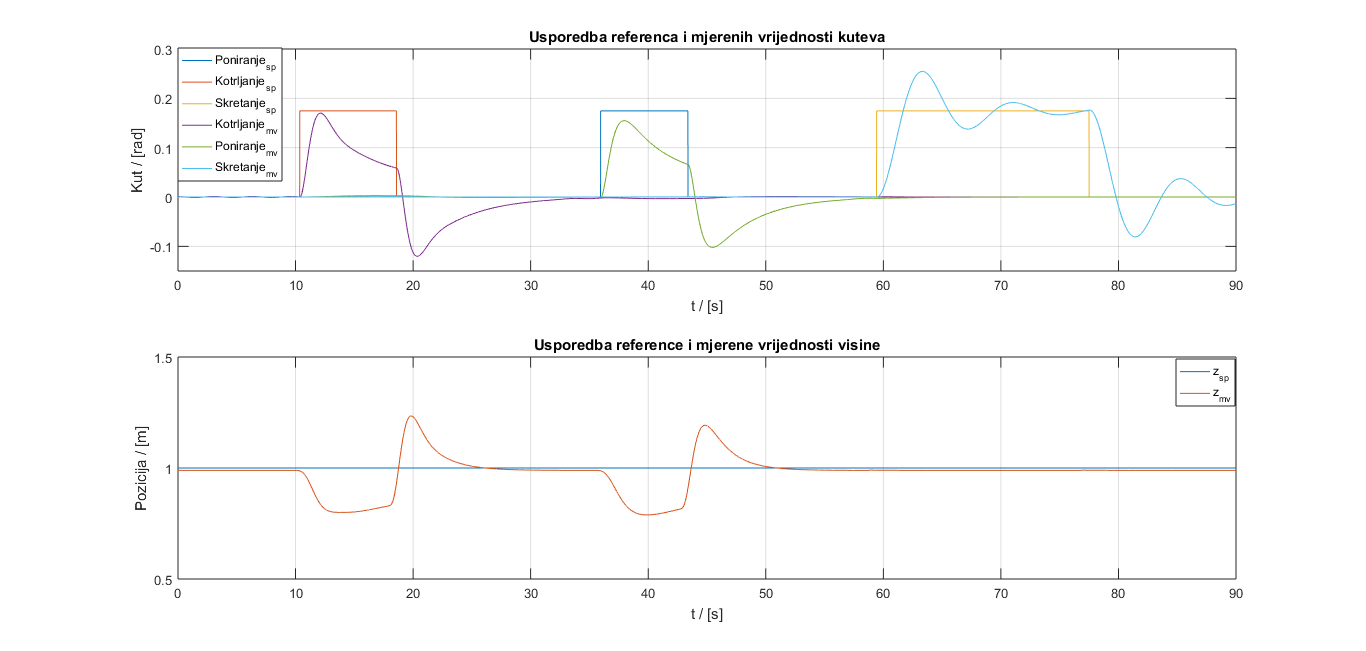
\includegraphics[width=\textwidth]{plots/orientation_euler.png}
		\caption{Prikaz odziva kuteva na skokovitu pobudu.}
	\end{figure}
	
	\newpage
	\clearpage
	
	\begin{figure}[h!]
		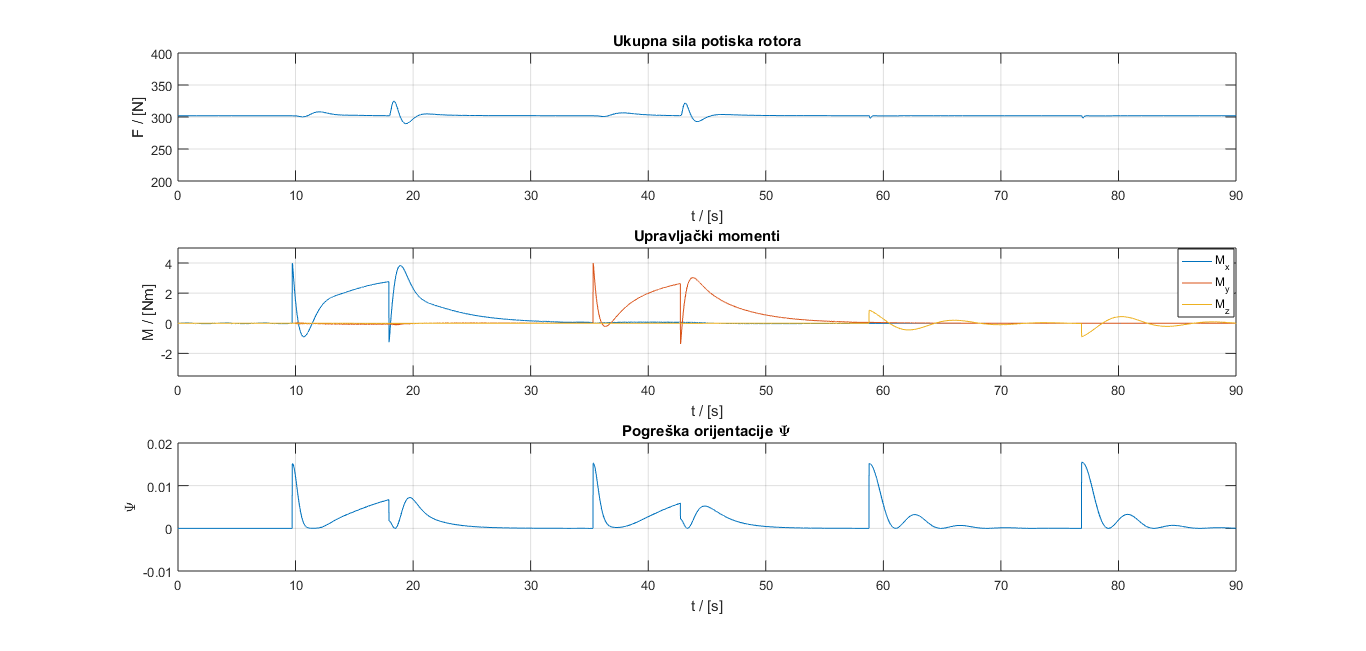
\includegraphics[width=\textwidth]{plots/orientation_forces_moments.png}
		\caption{Prikaz upravljačkih vrijednosti sila i momenata te pogreške orijentacije tokom zadavanja skokovite pobude kuteva.}
	\end{figure}
	Može se primijetiti kako prijelazna pojeva kuteva poniranja i valjanja je pristojna, ali nakon dostizanja referentne vrijednosti dolazi do izrazitog odstupanja u stavionarnom stanju. Ista stvar se dešava kod mjerene vrijednosti visine. U trenutku djelovanja na pobude kuteva, letjelica počinje gubiti na visini, odnosno dolazi do odstupanja a u stacionarnom stanju.
	
	\section{Slijeđenje trajektorije u pozicijskom načinu upravljanja}
	U ovom dijelu bit će prikazana spiralna trajektorije uz dodatak rotacije oko z-osi. Slijeđenje trajektorije podrazumijeva zadavanje željene pozicije, željene brzine i akceleracije te smjera x-osi letjelice.
	
	\begin{figure}[h!]
		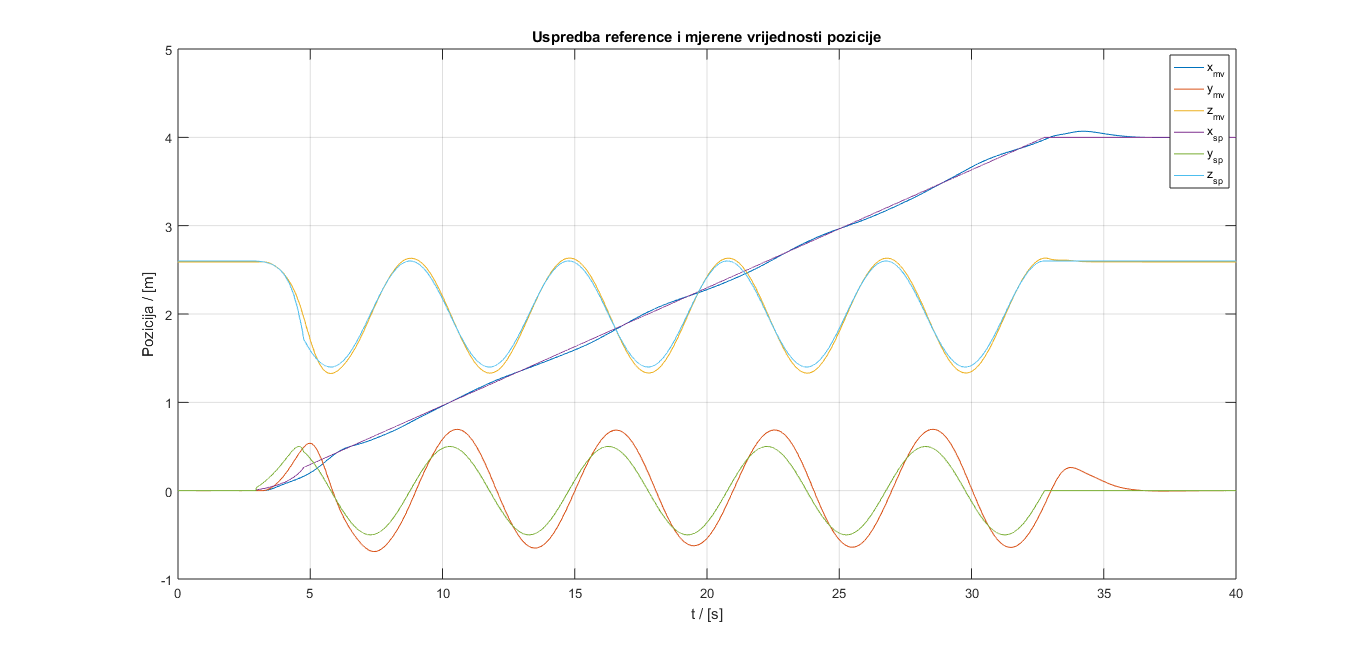
\includegraphics[width=\textwidth, height=7cm]{plots/traj_pos2.png}
		\caption{Prikaz odziva pozicije letjelice na zadanu trajektoriju.}
	\end{figure}
	
	\newpage
	\clearpage
	
	\begin{figure}[h!]
		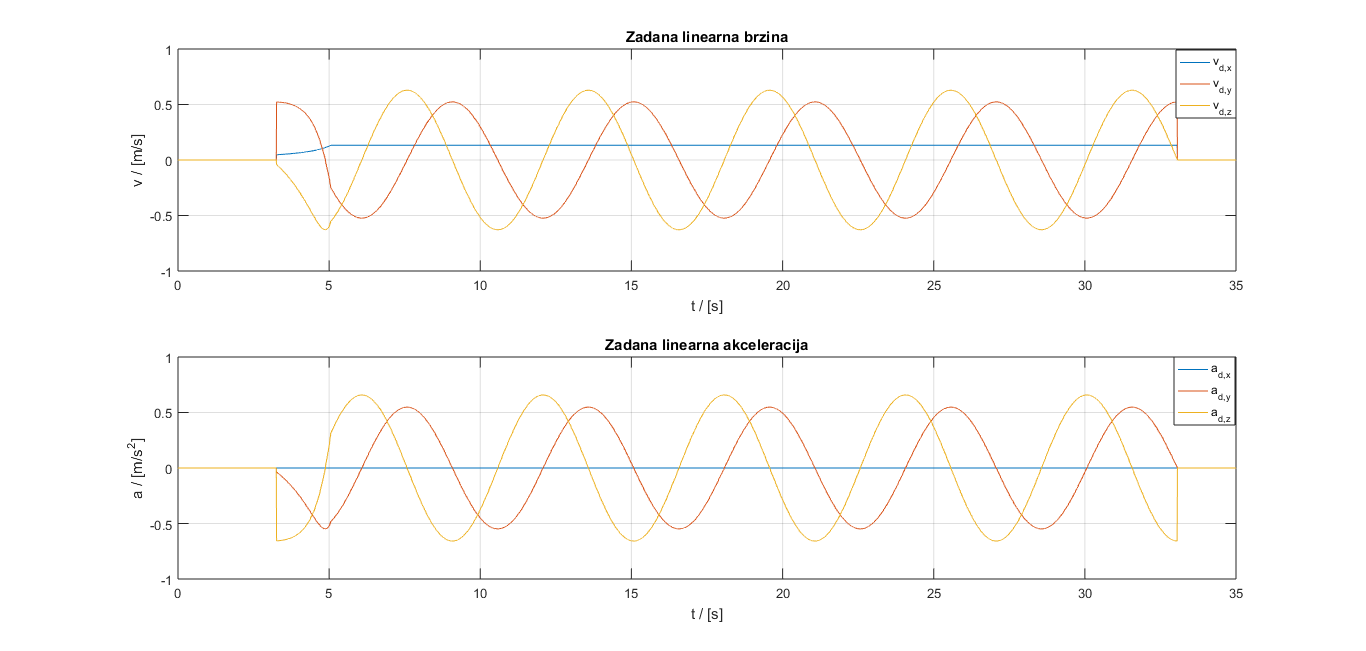
\includegraphics[width=\textwidth]{plots/traj_a_v2.png}
		\caption{Prikaz željenih vrijednosti linearne brzine i akceleracije, izračunatih direktno iz poznatog signala trajektorije.}
	\end{figure}
	
	\begin{figure}[h!]
		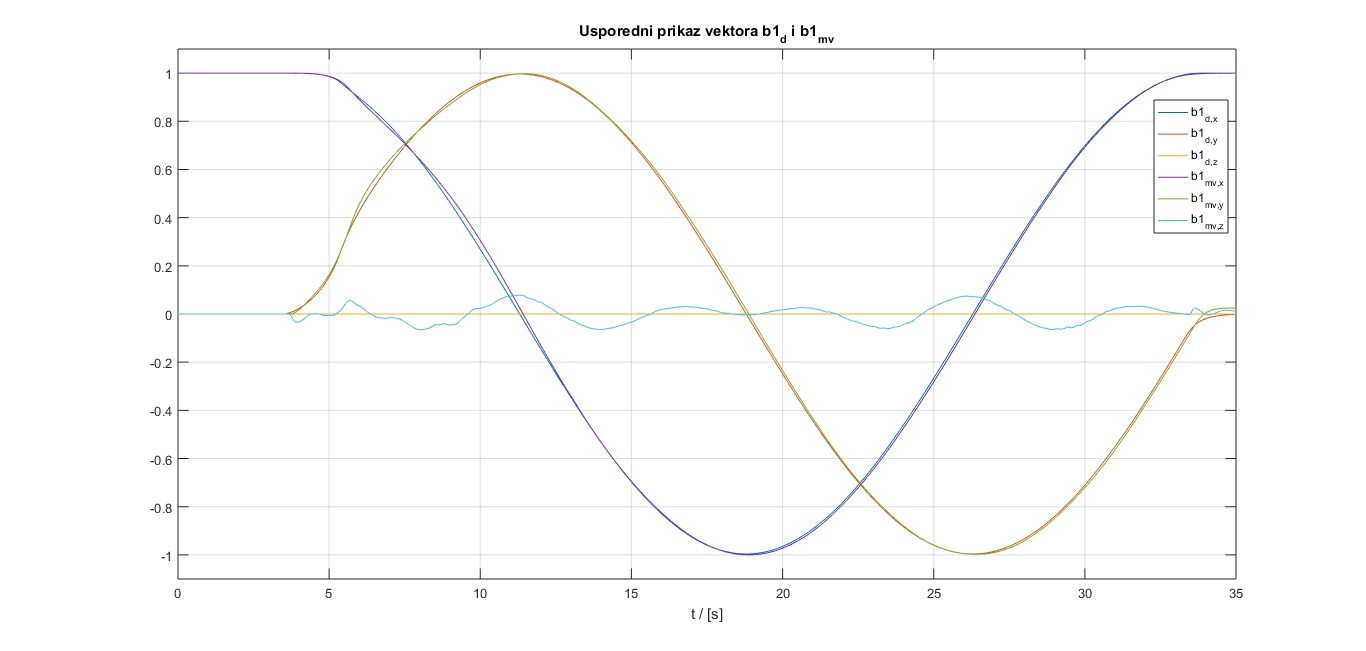
\includegraphics[width=\textwidth]{plots/traj_b1d2.png}
		\caption{Prikaz odziva smjera x-osi letjelice na zadanu trajektoriju. }
	\end{figure}
	
	Jednadžba trajektorije je slijedeća:
	\begin{gather}
		x(t) = 0.4t \label{traj_x}\\
		y(t) = 0.5 sin(\pi t) \label{traj_y}\\
		z(t) = 0.6 cos(\pi t) + 2 \label{traj_z}\\
		b1_{d,x}(t) = cos(\pi t / 5) \\
		b1_{d,y}(t) = sin(\pi t / 5) \\
		b1_{d,z}(t) = 0
	\end{gather}
	\begin{figure}[h!]
		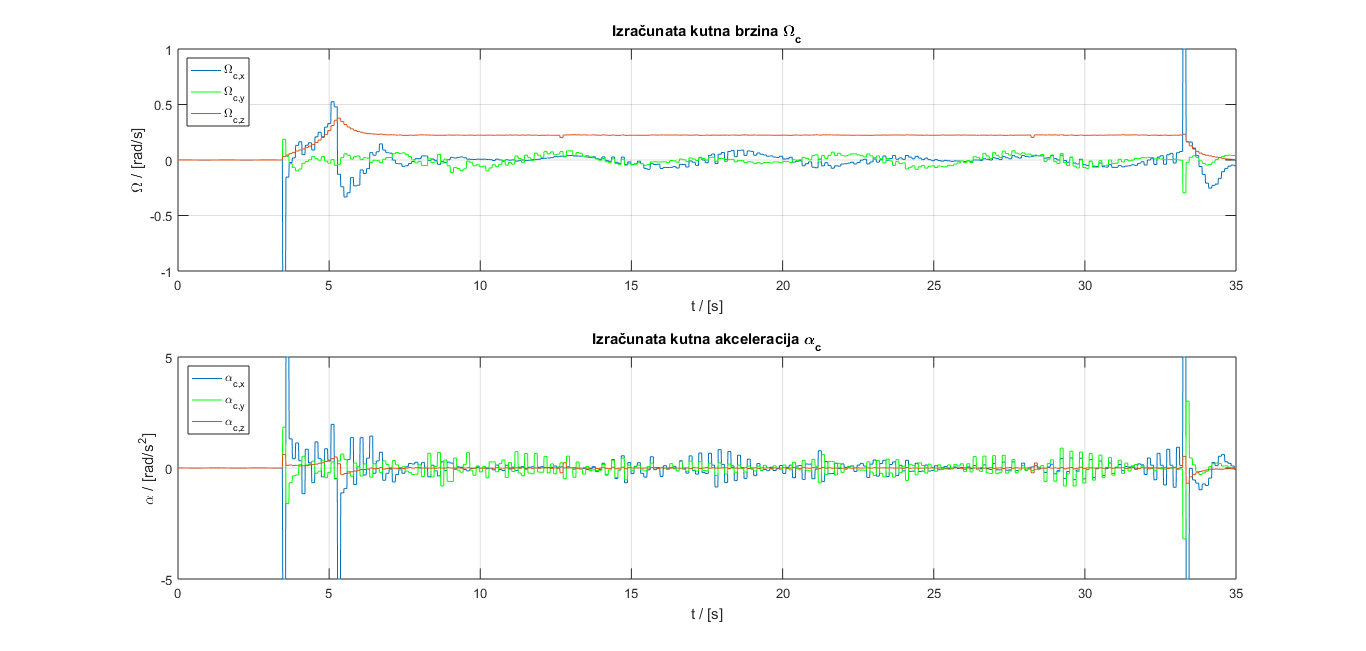
\includegraphics[width=\textwidth]{plots/traj_alpha_omega2.png}
		\caption{Prikaz izračunatih vrijednosti kutne brzine i akceleracije tijekom zadane trajektorije.}
	\end{figure}
	
	\begin{figure}[h!]
		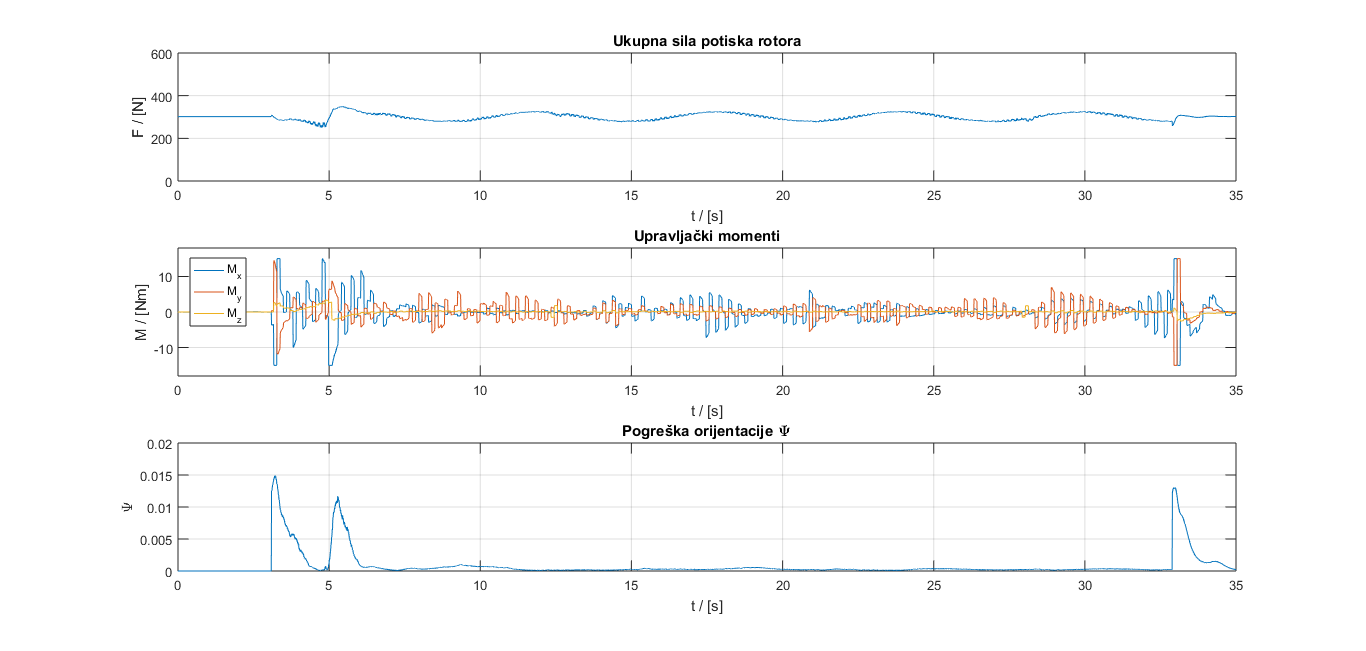
\includegraphics[width=\textwidth]{plots/traj_force_moments2.png}
		\caption{Prikaz upravljačkih vrijednosti sila i momenata te pogreške orijentacije tokom trajektorije.}
	\end{figure}
	
	Inicijalno napravljena je trajektorija u trajanju od 10 sekundi međutim radi trome prirode letjelice trajektorija je usporena 3 puta. Rotacija oko z-osi je također značajno usporena.\\
	Željene brzine i akceleracije izračunate su deriviranjem izraz za poziciju \ref{traj_x}, \ref{traj_y} i \ref{traj_z}. Vrijednosti željene brzine i akceleracije skalirane su odgovarajućim faktorom budući da je ukupna trajektorija nekoliko puta usporena.
	
\chapter{Zaključak}
	\paragraph{} Prilikom slijeđenja trajektorije geometrijsko upravljanje pokazalo se zadovoljavajućim. Najveći problem javlja se prilikom rotacije letjelice oko z-osi što se može objasniti velikom tromošću samog tijela letjelice te zbog samih benzinskih motora. Naime, unutar simulacije imaju ugrađenu vremensku konstantu prijelazne pojave brzine vrtnje rotora što znači da upravljačke sile ne djeluju trenutno na tijelo letjelice. 
	\todo[inline]{napisati jos nesto...}
	
\chapter{Dodatak}
	\section{Funkcije pogreške u SO(3) prostoru}
	
	U izvodu se koriste slijedeći Lijevi identiteti:
	\begin{gather}
		A\in so(3), \,  x\in\mathbb{R}^3 \\
		A^T = -A \\
		R \hat{x}R^T = (Rx)^\wedge \\
		tr(R\hat{x}) = - (A - A^T)^\text{V} \cdot x
	\end{gather}
	\begin{align*}
		\frac{d}{dt}\Psi(R, R_d) &= \frac{d}{dt} ( \frac{1}{2} tr(I - R_d^TR)) \\
		&= - \frac{1}{2}tr(\dot{R}_d^TR + R_d^T\dot{R}) \\
		&= - \frac{1}{2}tr( (R_d \hat{\Omega_d})^TR + R_d^TR\Omega ) \\
		&=  - \frac{1}{2}tr( -\hat{\Omega_d}R_d^TR + R_d^TR\hat{\Omega}) \\
		&= - \frac{1}{2}tr[ -R_d^TR \, (R^TR_d\hat{\Omega}_dR_d^TR) + R_d^TR\hat{\Omega} ] \\
		&=  - \frac{1}{2}tr[ -R_d^TR \, (R^TR_d\Omega_d)^\wedge + R_d^TR\hat{\Omega} ] \\
		&= - \frac{1}{2}tr[ -R_d^TR (\Omega - R^TR_d\Omega_d)^\wedge ] \\
		&= \frac{1}{2}(R_d^TR - R^TR_d)^\text{V} \cdot (\Omega - R^TR_d\Omega_d) \\
		&= e_R \cdot e_\Omega
	\end{align*}
	
	U posljednje dvije linije može se prepoznati izraz \ref{error}. Stoga je prvi faktor uzet kao pogreška konfiguracije, a drugi kao pogreška brzine slijeđenja.
	
	\newpage
	\clearpage
	
	\section{Pozicijski način upravljanja}
	Kako bi se odabrao upravljački zakon \ref{thrust_ctrl} najprije je potrebno napisati dinamiku pogreške linearne brzine \ref{e_v}. Zatim odabrati zadovoljavajući upravljački zakon te analizom stabilnosti pokazati kako je ta pogreška stabilna.
	
	\begin{gather*}
		e_v = v - v_d \,/ \cdot m \\
		me_v = mv - mv_d \, / \cdot \frac{d}{dt} \\
		m\dot{e}_v = m \ddot{x} - m\ddot{x}_d
	\end{gather*}
	Sada se u gornji izraz uvrštava jednadžba gibanje \ref{thrust_dyn} iz čega slijedi:
	\begin{equation}
		m\dot{e}_v = mge_3 - fRe_3 - m\ddot{x}_d \label{dyn_v}
	\end{equation}
	Neka je $A\in\mathbb{R}^3$ željena upravljačka veličina potiska. Tada vrijedi:
	\begin{gather}
		A = \Vert A \Vert R_d e_3 \\
		f = - A \cdot Re_3
	\end{gather}
	U svrhu ugrađivanja pogreške orijentacije u dinamiku pogreške brzine, izrazu \ref{dyn_v} dodaje i oduzima se slijedeći izraz:
	\begin{equation}
		\frac{f}{(R_de_d)^TRe_3}R_d e_3 = \frac{\Vert A \Vert R_d e_3 \cdot Re_3}{(R_de_d)^TRe_3}\frac{A}{\Vert A \Vert} = - A
	\end{equation}
	
	Izraz \ref{dyn_v} sada poprima slijedeći oblik:
	\begin{align*}
		m\dot{e}_v =& m \ddot{x} - m\ddot{x}_d \\
		& + \frac{f}{(R_de_d)^TRe_3}R_d e_3 - \frac{f}{(R_de_d)^TRe_3}R_d e_3 \\
		& - \frac{f}{(R_de_d)^TRe_3}((R_de_d)^TRe_3)Re_3 \\
	\end{align*}
	Ako se sada uvede nova varijabla $X$ koja će sadržavati 3. i 5. član gornjeg izraza tada se gornja jednadžba pojednostavljuje na:
	\begin{equation*}
		m\dot{e}_v = mge_3 - m\ddot{x}_d + A + X
	\end{equation*}
	Sada se upravljački zakon $A$ odabire na način da se kompenzira dinamika sustava: 
	\begin{gather}
		A = -k_x e_x - k_ve_v - mge_3 + m\ddot{x}_d \\
		m\dot{e}_v = -k_x e_x - k_v e_v + X \label{lin_dyn}
	\end{gather}
	
	\newpage
	\clearpage
	
	Analogno, kako bi se odabrao upravljači moment najprije je napisati jednadžbu dinamike pogreške kutne brzine \ref{e_omega}. Zatim odabrati odgovarajući upravljački zakon te analizom stabilnosti pokazati kako je ta pogreška stabilna.
	\\ Uz slijedeća svojstva:
	\begin{gather}
		(Ax)^\wedge = A\hat{x}A^T \\
		\hat{\Omega}\Omega = 0 \, , \Omega\in so(3)
	\end{gather}
	vrijedi:
	\begin{align*}
		\frac{d}{dt} e_\Omega &= \dot{\Omega} - \left(\frac{d}{dt}(R^TR_d)\Omega_d + R^TR_d\dot{\Omega}_d\right) \\
		&= \dot{\Omega} - ( (R_d^TR\hat{e}_\Omega)^T\Omega_d + R^TR_d\dot{\Omega}_d) \\
		&= \dot{\Omega} - (-\hat{e}_\Omega R^TR_d\Omega_d + R^TR_d\dot{\Omega}_d)\\
		&= \dot{\Omega} - (- (\hat{\Omega} - (R^TR_d\Omega_d)^\wedge)R^TR_d\Omega_d + R^TR_d\dot{\Omega}_d)\\
		&= \dot{\Omega} - (- \hat{\Omega}R^TR_d\Omega_d + (R^TR_d\Omega_d)^\wedge R^TR_d\Omega_d + R^TR_d\dot{\Omega}_d)\\
		&= \dot{\Omega} - (- \hat{\Omega}R^TR_d\Omega_d + R^TR_d\Omega_d\Omega_d + R^TR_d\dot{\Omega}_d) \\
		&= \dot{\Omega} + \hat{\Omega}R^TR_d\Omega_d - R^TR_d\dot{\Omega}_d
	\end{align*}
	Ako se sada u gornju dinamiku pogreške uvrsti izraz \ref{e_omega} dobije se slijedeće:
	\begin{gather*}
		\dot{e}_\Omega = \dot{\Omega} + \hat{\Omega}R^TR_d\Omega_d - R^TR_d\dot{\Omega}_d / \cdot J\\
		J\dot{e}_\Omega = J \dot{\Omega} + J(\hat{\Omega}R^TR_d\Omega_d - R^TR_d\dot{\Omega}_d) \\
		J\dot{e}_\Omega = M - \Omega \times J\Omega + J(\hat{\Omega}R^TR_d\Omega_d - R^TR_d\dot{\Omega}_d)
	\end{gather*}
	Izraz za M se sada odabire na način da se kompenzira dinamika pogreške:
	\begin{equation}
		M = -k_R e_R - k_\Omega e_\Omega + \Omega \times J \Omega - J(\hat{\Omega}R^TR_d\Omega_d - R^TR_d\dot{\Omega}_d) \label{M_u}
	\end{equation}
	Uvrštavanje \ref{M_u} u izraz za dinamiku pogreške dobije se:
	\begin{equation}
		J\dot{e}_\Omega = -k_R e_r - k_\Omega e_\Omega \label{ang_dyn}
	\end{equation}
	
	\noindent Upućuje se na \cite{2010arXiv1003.2005L}, \cite{5717652}, \cite{2011arXiv1109.4457L} za uvid u provedbu analize stabilnosti Ljapunovljevom metodom. 
	
	\newpage
	\clearpage
	
	\section{Parametri regulatora}
	Postupak pronalaženja parametera regulatora proveden je sukladno sa predloženom metodom u \cite{zavrsniCirjak}.
	Početni parametri regulatora određeni su analiziranjem izrazima za dinamiku linearne i kutne pogreške \ref{lin_dyn}, odnosno  \ref{ang_dyn}. Ako se pretpostavi da je orijentacija letjelice u početnom stanju, te da vrijedi $\dot{e}_R=e_\Omega$ tada se dobiju slijedeće diferencijalne jednadžbe drugog reda:
	\begin{gather}
		\ddot{e}_x + \frac{k_v}{m}\dot{e}_x + \frac{k_x}{m}e_x = 0 \\
		\ddot{e}_R + \frac{k_\Omega}{J}\dot{e}_R + \frac{k_R}{J}e_R = 0
	\end{gather}
	
	\noindent Uspoređujući navedene jednadžbe sa karakterističnom prijenosnom funkcijom PT2S člana: 
	\begin{equation}
		s^2 + 2 \zeta \omega_n s + \omega_n^2 = 0
	\end{equation}
	dobiju se slijedeći parametri regulatora:
	\begin{gather}
		k_x = \omega_n^2 m \\
		k_v = 2 \zeta \omega_n m \\
		k_R = \omega_n^2 J \\
		k_\Omega = 2 \zeta \omega_n J
	\end{gather}
	Faktor prigušenja uzet je jednak za sve slučajeve i iznosi $\zeta = \frac{\sqrt{2}}{2}$. \\
	Za $k_x$ i $k_v$ uzeta je prirodna frekvencija $\omega_n = 2 \, rad / s$ za x, y komponentu, a $\omega_n = 5 \, rad / s$ za z komponentu. Odabrana pojačanja iznose:
	\begin{equation}
		k_x = 
		\begin{bmatrix}
			120 & 0 & 0 \\
			0 & 120 & 0 \\
			0 & 0 &  714 
		\end{bmatrix}
		\, , \, 
		k_v = 
		\begin{bmatrix}
			84 & 0 & 0 \\
			0 & 84 & 0 \\
			0 & 0 & 285
		\end{bmatrix}
	\end{equation}
	Pojačanjima za proporcionalnu i derivativnu komponentu visine dodana je dodatna korekcija zbog odstupanja u stacionarnom stanju.\\
	Kod pojačanja $k_R$ i $k_\Omega$ uzeta je prirodna frekvencija $\omega_n = 2 \, rad/s$ za x, y komponentu, a $\omega_n = 5 \, rad/s$ za z komponentu. Odabrana pojačanja iznose:
	\begin{equation}
		k_R = 
		\begin{bmatrix}
			23.04 & 0 & 0 \\
			0 & 23.04 & 0 \\
			0 & 0 & 5
		\end{bmatrix}
		\, , \,
		k_\Omega = 
		\begin{bmatrix}
			16.29 & 0 & 0 \\
			0 & 16.29 & 0 \\
			0 & 0 & 2.5
		\end{bmatrix}
	\end{equation}
	Kao i u prethodnom slučaju pojačanja z-komponente dodatno su korigirane radi boljeg odziva kuta skretanja letjelice.
	
\begin{sazetak}
Ravijen je nelinearni geometrijski regulator za upravljanje multirotorskom letjelicom s benzinskim motorima. Regulator je implementiran u programskom jeziku C++ u ROS okruženju te ispitan korištenjem simulacijskog okruženja Gazebo na postojećem modelu multirotorske bespilotne letjelice s benzinskim motorima i pokretnim masama.

\kljucnerijeci{geometrijsko upravljanje, multirotorska letjelica, Lijeve grupe, SE(3), ROS, Gazebo}
\end{sazetak}

% TODO: Navedite naslov na engleskom jeziku.
\engtitle{Title}
\begin{abstract}
A nonlinear geometric controller is implemented using C++ programming language within ROS environment. The controller is used on a multirotor unmanned aerial vehicle with internal combustion engines. Results are obtained from Gazebo simulation environment using the existing multirotor UAV model with internal combustion engines and moving masses.

\keywords{geometric control, multirotor UAV, Lie groups, SE(3), ROS, Gazebo}
\end{abstract}

\nocite{*}
\bibliography{literatura}
\bibliographystyle{fer}

\end{document}